\chapter{Подавление артефактов, вызванных наличием сильнопоглощающих включений} \label{chapt2}
\section{Введение}

В данной главе рассматривается задача исправления ошибок реконструкции, возникающих при томографии сложных объектов, содержащих области сильного поглощения рентгеновского излучения.
Наличие подобных артефактов (рис. \ref{im:high_absorb_artifacts}) сильно затрудняет последующий анализ результатов томографии.
Поэтому необходимо использовать алгоритмы, учитывающие специфику исследуемого объекта и позволяющие уменьшить влияние сильнопоглощающих включений на результаты восстановления.
Часто такие артефакты возникают при анализе медицинских изображений, если в костях или мягких тканях объекта присутствуют металлические включения.
Например в стоматологии, металлический штифт, необходимый для установки коронки, может быть причиной возникновения ложных полостей в зубе, что может быть причиной неправильного решения об успешности проведенного лечения.
Поэтому такие артефакты так же называют металлическими, хотя они могут возникать в объектах разного состава при соответствующих интенсивности истоячника и чувствительности детектора.
Термин ``сильнопоглощающие'' применим к более широкому набору условий экспериментов, но часто артефакты все равно называют металлическими.


Обычно для подавления этих артефактов на алгоритмическом уровне используют методы, основанные на предобработке синограммы, модификации алгебраических методов на основе методов максимального правдоподобия или выпуклого программирования.
В данной главе будут исследованы методы подавления металлических артефактов на этапе алгоритма восстановления.
Первый метод, предложенный и реализованный автором, использует математический аппарат квадратичного программирования в рамках специально построенной модели формирования металлических артефактов.
Возникновение артефактов в ней выражается в виде неучтенных при восстановлении линейных ограничений-неравенств, которые в купе с квадратичной функцией потерь исходной оптимизационной задачи алгебраического метода и позволяют использовать аппарат численной условной оптимизации.
Второй метод, реализованный Соколовым В., основываясь на той же модели формирования артефактов, решает задачу восстановления путем добавления аддитивных мягких ограничений за нарушение неравенств модели.
Автором была произведена настройка параметров метода и получение приведенных в главе результатов.
Наконец, производится сравнение результатов восстановления обоих методов на модельном примере.

\begin{figure}
\centering
\begin{tabular}{@{}c@{}c}
  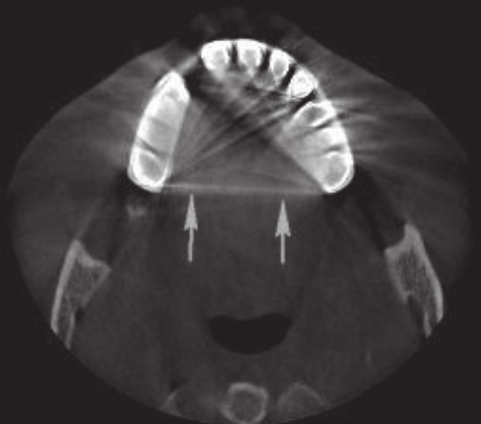
\includegraphics[width=0.3\textwidth]{part2_img/tooth_artifacts_med}
  &
  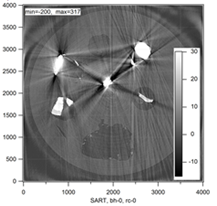
\includegraphics[width=0.3\textwidth]{../Presentation/images/high_absorb_artifacts}
\\
\end{tabular}
\caption{Примеры артефактов, вызванных наличием сильнопоглощающих включений в объекте}
\label{im:high_absorb_artifacts}
\end{figure}

Далее структура главы будет следующая: сначала будет приведено описание модели и метода восстановления на основе примера малой размерности.
Затем - приведен способ продолжить полученные результаты для входных данных большей резмерности.
После этого приведено описание метода восстановления на основе мягких ограничений.
Наконец, будут обсуждены полученные результаты и сделаны выводы.

Основной вклад данной главы состоит в следующем: предлагается модель формирования артефактов, вызванных наличиием сильнопоглощающих включений, предлагается метод восстановления на основе данной модели, исследуются результаты работы данного метода на различных входных данных, а также производится сравнение результатов восстановления методов, основанных на квадратичном программировании и на использовании ``мягких'' аддитивных квадратичных штрафов. 
Все предложенные алгоритмы в главе сопровождаются вычислительным экспериментом, результаты которых анализируются в соответствующем разделе.

\section{Модель возникновения артефактов}
\label{sect_2_0}

Предлагаемая модель основывается на предположении о некорректной интерпретации измеренных данных, и в результате неправильно построенной задаче оптимизации для нахождения восстеновленного изображения.
Ренгеновское излучение, проходя через металлическое включение, ослабляется сильнее чем в остальных областях исследуемого образца.
В результате в пиксели детектора, соответствующие высокопоглощающим областям под данным углом проекции, попадает излучение интенсивностью, сравнимой с уровенем шума.
В этом случае измерение будет излишне зашумлено, то есть соотношение сигнал-шум неприемлемо для восстановления, либо после прохождения АЦП в измерениях с этих лучей будет записано значение 0.
Однако все что можно сказать про эти измерения, это что реальное значение в них лежит где-то в интервале $[0, \delta_{min})$, где $\delta_{min}$ --- минимальный порог срабатывания детектора, или уровень шума.
Поэтому и восстановление измерений для этих лучей неоходимо производить отдельно, учитывая механизм их возникновения.

Предлагаемая модель может быть выражена в оптимизационной задаче алгебраического метода в виде ограничений-неравенств.
После обычной для томографии процедуры логарифмирования условие для пикселей $j$ в которых интенсивность пришедшего излучения меньше порога ($I_j < \delta_{min}$) можно записать условие $P_j > \ln\frac{I_0}{\delta_{min}} = \delta$.
Учитывая, что в терминах алгебраического метода $P_j = \sum_i f_i w_{ij}$, оптимизационная задача с учетом предложенной модели будет выглядеть следующим образом:

\begin{equation}
  \label{eq:quadprog_ineq}
  \begin{cases}
  \Norm{P^{\textup{изм.}} - W(f)} \rightarrow \min\limits_f & w.r.t \\
  \sum_i f_{i} w_{ij} > \delta, & \mbox{если } P^{\textup{изм.}}_j = \delta \\
  f_{i} \geq 0
  \end{cases}
\end{equation}

В условия-неравенства оптимизационной задачи \eqref{eq:quadprog_ineq} так же введены условия-ограничения на неотрицательность значений логарифма линейной функции плотности поглощения рентгеновского излучения $f_i$.
Так как функционал ошибки квадратичный, а ограничения - линейные, для решения этой минимизационной задачи эффективным будет применить метод квадратичного программирования.
При этом в формулировке оптимизационной задачи присутствует полная матрица преобразования Хафа $w_{ij}$.
Как и в случае с алгебраическим методом, решение задачи возможно при использовании итеративной градиентной минимизации, ввиду ее огромной размерности.
Действительно, количество элементов матрицы приблизительно составляет $\sqrt{2} * n * n_\varphi \times n * n$ для изображения размером $n \times n$ и $n_\varphi$ проекционных углов.
При этом ненулевые значения для каждого столбца находятся только в $\approx n$ ячейках, делая возможным использование инструментария для работы с разреженными матрициы.
Несмотря на это, при $n = 256, n_\varphi = 180$ и использовании чисел с плавающей точкой двойной точности (тип данных float64) и способа хранения разреженных матриц ``compressed sparse row'' такая матрица в оперативной памяти вычислителя будет занимать порядка 170Мб.
При этом для традиционных методов решения задачи QP требуется рассчет обратного гессиана целевой функции, то есть матрицы $W W^{\mathrm{T}}$, которая в разреженном виде занимает 11Гб в оперативной памяти и ее невозможно обрабатывать стандартными реализациями ПО для режения задач выпуклого и квадратичного программирования.
Поэтому необходима разработка специальной процедуры, не требующей работы в явном виде с матрицами таких больших размерностей, а лишь с результатами ее умножения на вектор, которое можеь быть вычислено с помощью алгоритмов обработки изображений.

Дальнейшая структура главы следующая: сначала на изображениях малого разрмера будет показана применимость подхода, основанного на предложенной модели возникновения артефактов; после этого будут предложены два подхода к переносу результатов на изображения большего размера, и будет произведено сравнение этих подходов на модельном примере.

\section{Задача квадратичного программирования малой размерности}
\label{sect_2_1}

Для оценки применимости подхода, использующего условную оптимизацию для подавления металлических артефактов, рассматривается модельное распределение линейного коэффициента поглощения размера 10х10 пикселей, содержащее два объекта существенно разной поглощающей способности (рис. \ref{fig:qp_phantom_10by10} а).
Первый объект --- высокопоглощающая (металлическая) ``скобка'' слева фантома, второй --- ``крест'' из более прозрачного материала.
Ожидается что наличие металлического закрывающего объекта затруднит восстановление внутреннего мелкого объекта.
Синограмма данного фантома представлена на рис. \ref{fig:qp_phantom_10by10} б).

% \begin{figure}
%     \centering
%     \begin{tabular}{@{}c@{}c}
%     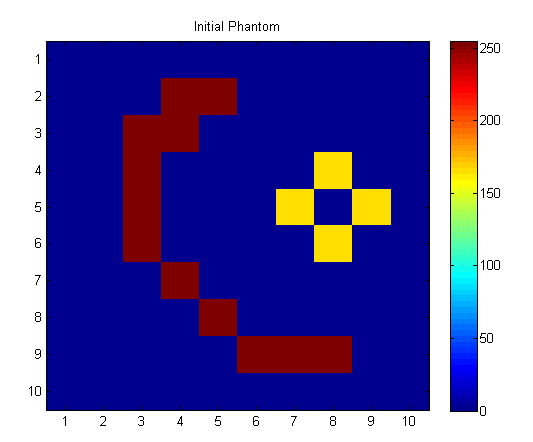
\includegraphics[width=0.4\textwidth]{../Presentation/images/qp_phantom} 
%     &
%     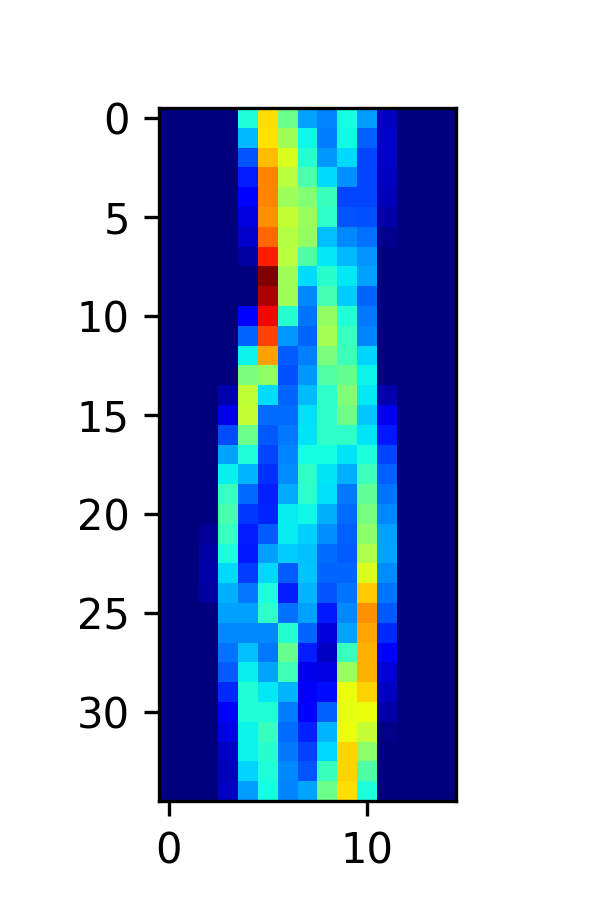
\includegraphics[width=0.4\textwidth]{../Presentation/images/qp_sino} 
%     \\
%     а) & б)
%     \end{tabular}
%     \caption{а) Модельный фантом размера 10х10 пикселей. б) синограмма}
%     \label{fig:qp_phantom_10by10}
% \end{figure}


\begin{figure}
    \centering
    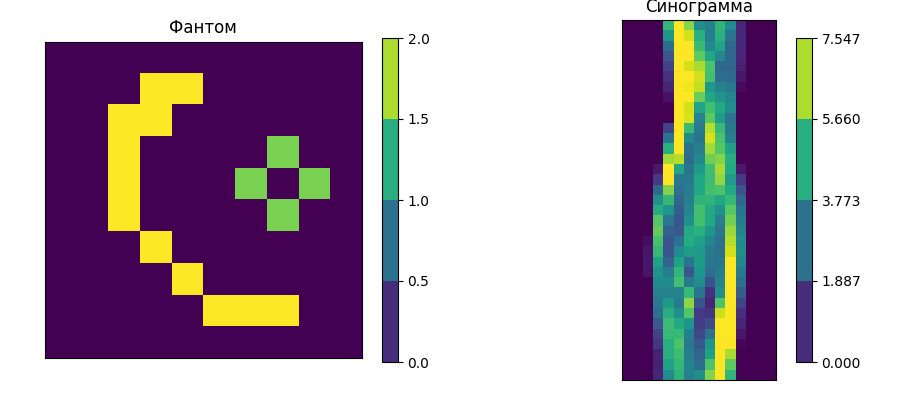
\includegraphics[width=0.9\textwidth]{part2_img/qp_input_10x10} \\
    а) \hspace{0.5\textwidth} б)
    \caption{а) Модельный фантом размера 10х10 пикселей. б) синограмма --- набор проекций данного фантома для 35 проекционных углов}
    \label{fig:qp_phantom_10by10}
\end{figure}

Порог $\delta$ для экспериментов подбирался таким образом, чтобы обрезать максимумы синограммы.
Значение порога было 800, размер пикселя был 1х1.
Значение сильнопоглощающего включение было 250, слабопоглощающего объекта - 160.
При расчете синограммы использовалось 35 проецкионых углов, равномерно распределенных в интервале от 0 до 180 градусов.

Для вычисления синограммы используется стандартная процедура прямой томографической проекции.
Однако для формирования входных данных для минимизации в задаче квадратичного программирования необходимо вычислить матрицу проекции $W$ поэлементно.

\section{Вычисление значений элементов матрицы проекции}

Действие оператора томографической поекции $W$ на дискретное изображение распределение линейного коэффициента поглощения $f$ легко вычисляется с помощью алгоритмов обработки изображений.
В этом параграфе  предстоит совершить ``обратное'' --- имея возможность делать прямую проекцию вычислить значения элементов матрицы $w_{ij}$
В данном разделе будет построен алгоритм вычисления элементов матрицы, используя декомпозицию оператора $W$ по отдельным лучам проекции а так же линейность самого преобразования томографической проекции.

Действие оператора проекции на изображение обозначается как $\mathbf{p} = W\mathbf{f}$.
Введем калибровочные изображения $\mathbf{f}^{(k)} = \delta_{ik}$, имеющие только один ненулевой пиксель.
За $\delta_{ik}$ обозначен символ Кронекера, т.е. тензор, значения которого удовлетворяют $\delta_{ik} = 1 \text{, если} i = j \text{, иначе } 0$.
Любое изображение на входе оператора проекции можно представить в виде линейной комбинации калиборочных: $\mathbf{f} = \sum_k f_k \mathbf{f}^{(k)}$.
Значит для вычисления элементов линейного оператора $W$ можно затабулировать результаты его применения ко всем калибровочным изображениям:

\begin{equation}
  \label{eq:w_on_calib_img}
  p_j = \left(W \mathbf{f}^{(k)} \right)_j = \sum_i w_{ij} \delta_{ik} = w_{kj}
\end{equation}

В результате алгоритм вычисления значений матрицы $W$ представлен в алг. \ref{alg:hough_matrix}:

\begin{algorithm}[H]
 \KwData{линейный размер входного изображения $n$, количество углов проекции $n_\varphi$}
 \KwResult{значения элементов матрицы $w_{ij}$}
 инициализация нулями матрицы (возможно, разреженной) $W \in \textbf{Mat}\left(nn, nn_\varphi)\right)$\;
 \For{каждого пикселя $k = 0 \dots nn$}{
  вычислить значение проекции калибровочного изображения $\mathbf{p}^{(k)} = W \mathbf{f}^{(k)}$\;
  обновить значение жлементов $w_{kj}$ используя формулу \eqref{eq:w_on_calib_img}\;
 }
 \caption{Алогритм вычисления элементов матрицы $w_{ij}$}
 \label{alg:hough_matrix}
\end{algorithm}

\todo{Подумать над тем, чтобы убрать эти иллюстрации в приложение} \\
Ниже (рис. \ref{fig:w_matrices}) приведены примеры вычислнных матриц для различных разрешений изображения и количества проекционных углов.

\begin{figure}
\centering
\begin{tabular}{c c c}
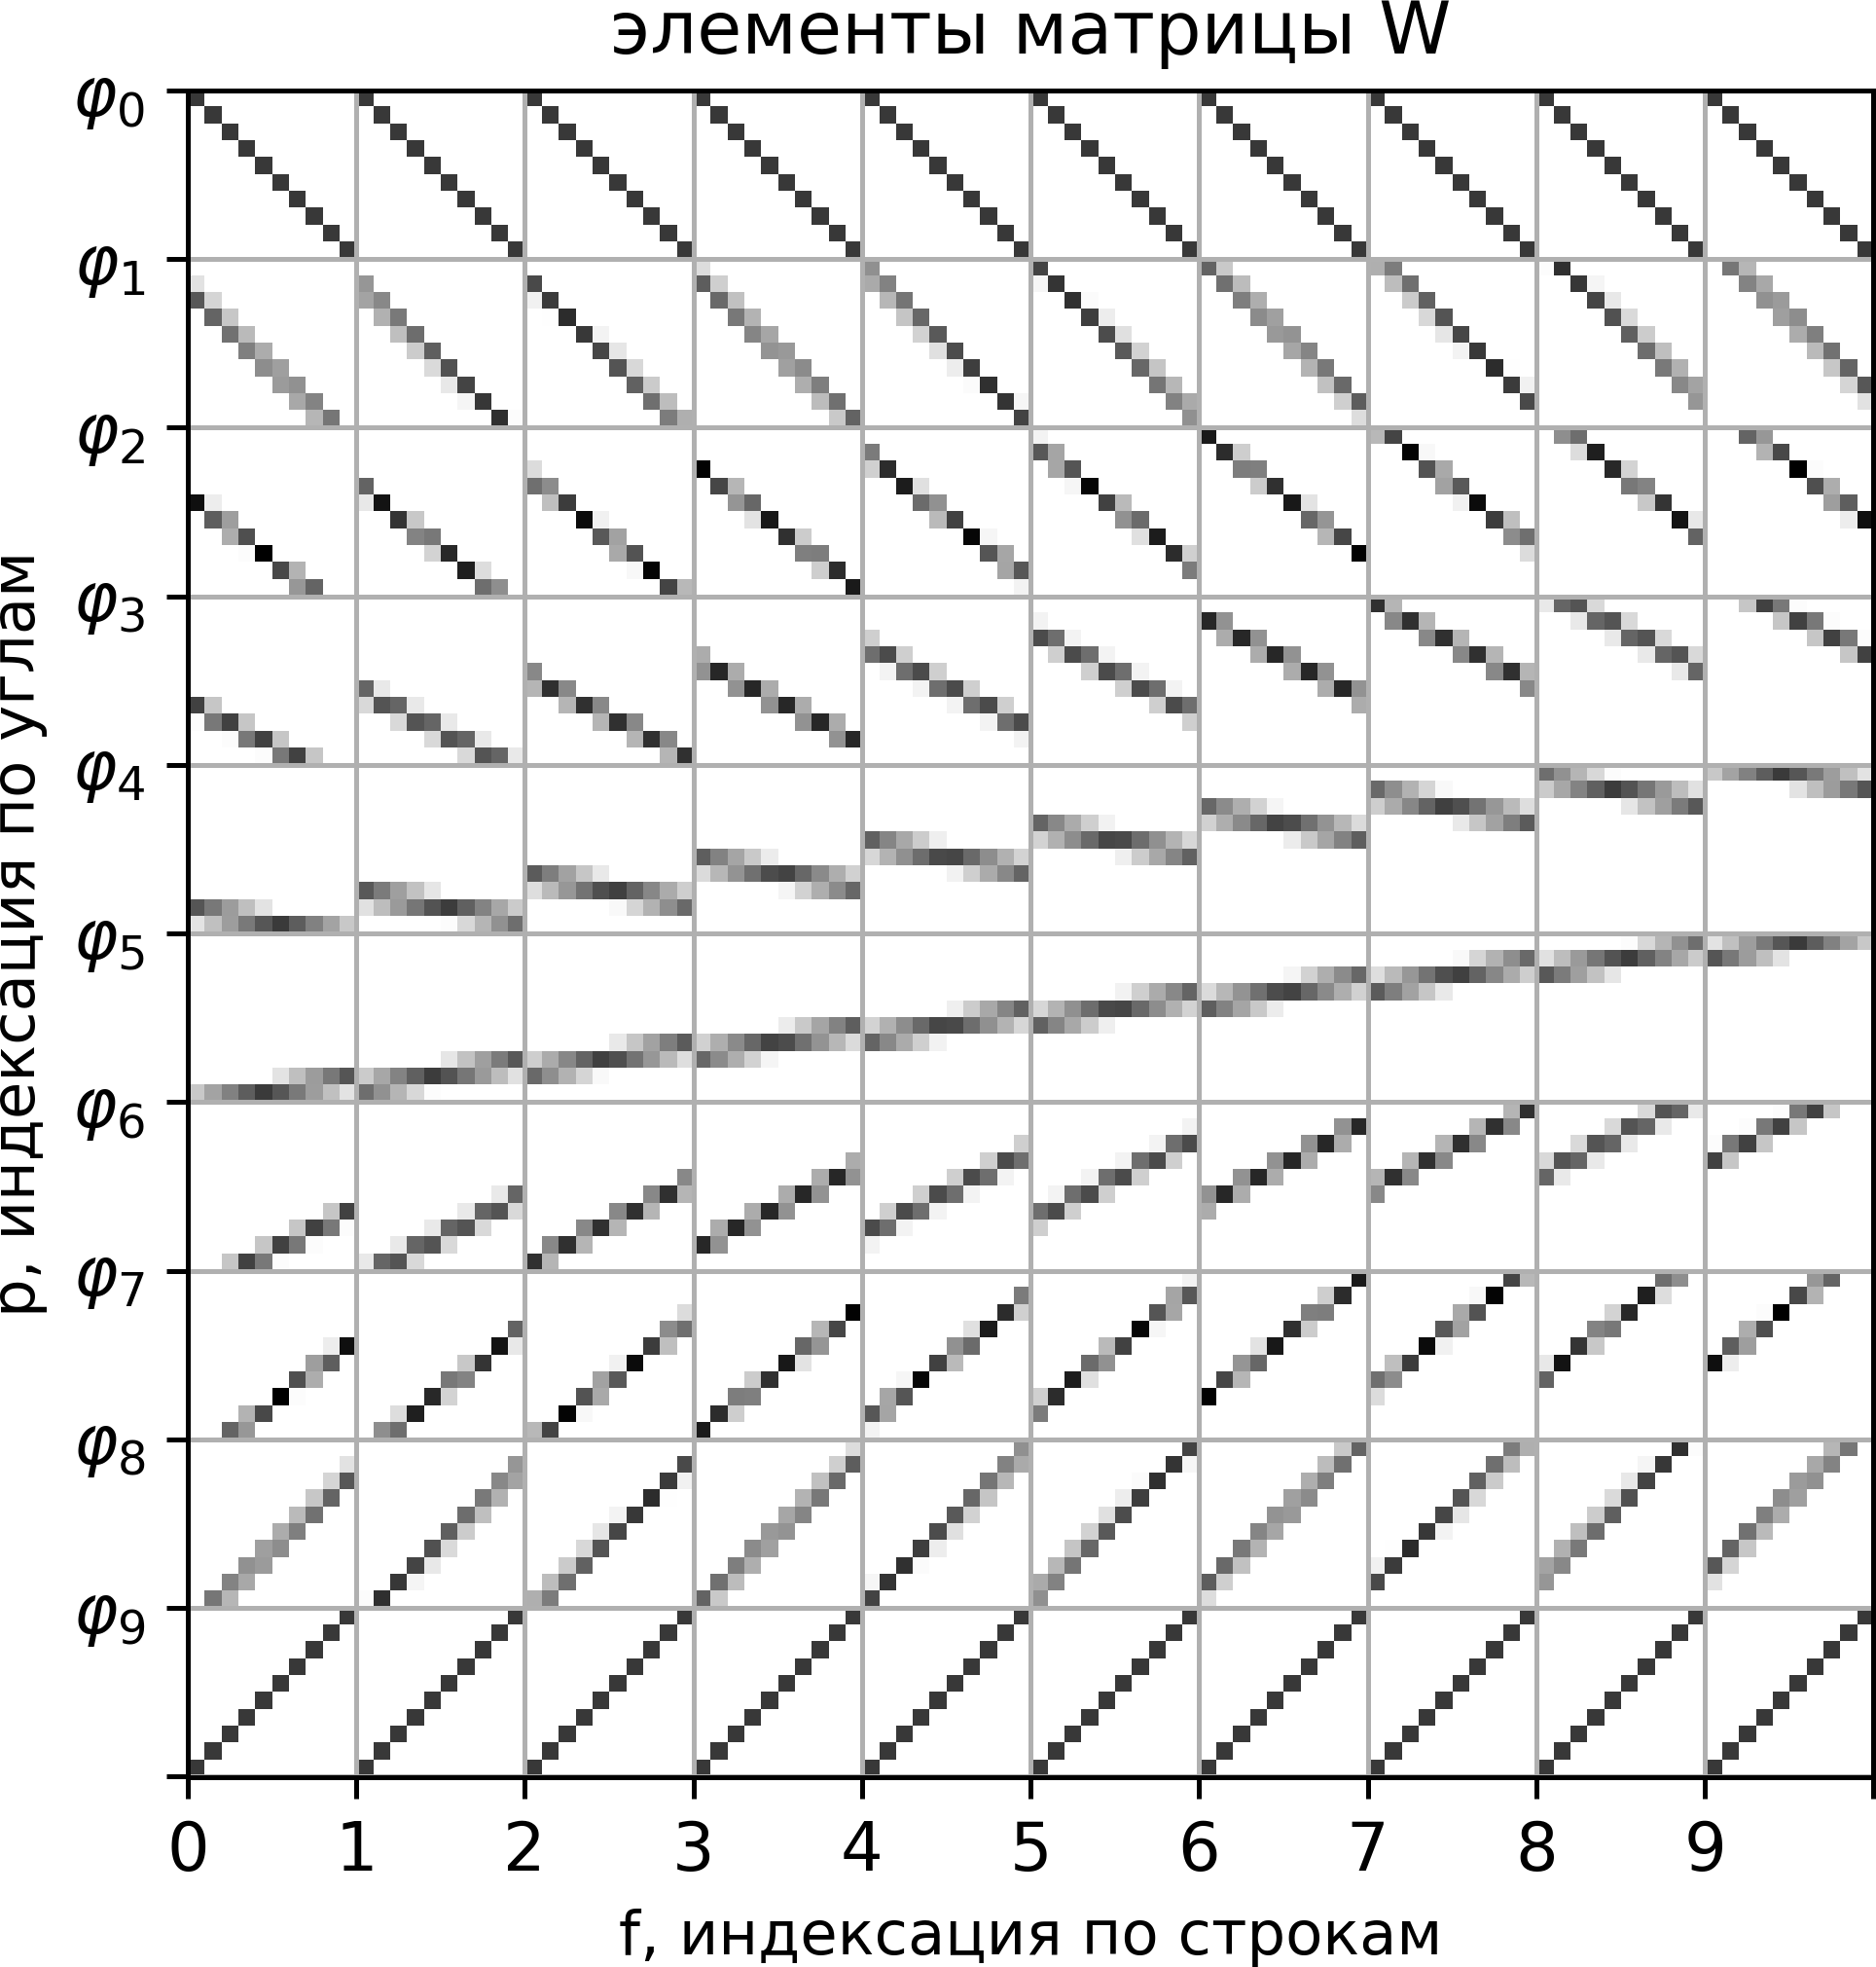
\includegraphics[width=0.35\textwidth]{../../Presentation/images/w_matrices/W_10_10_plot.png} &
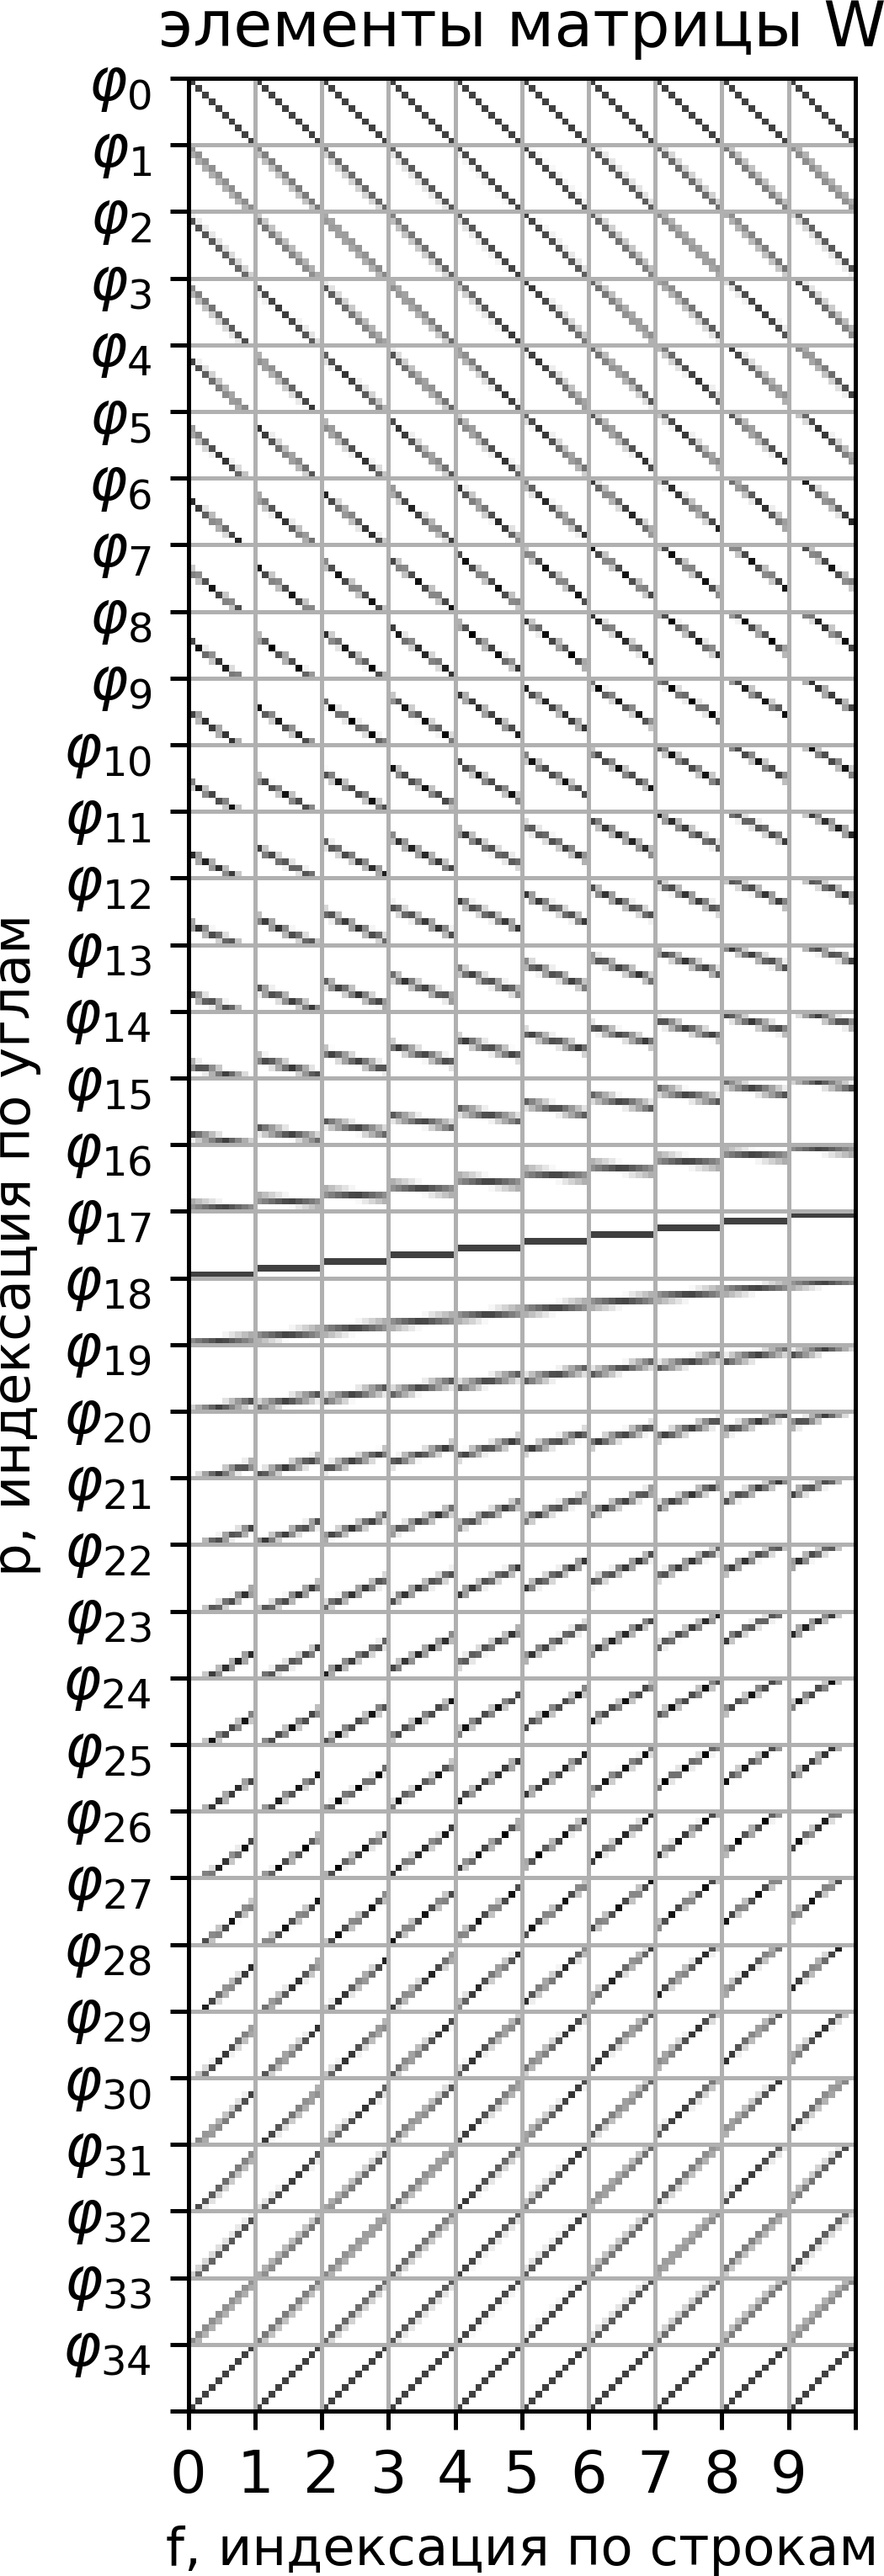
\includegraphics[width=0.25\textwidth]{../../Presentation/images/w_matrices/W_10_35_plot.png} &
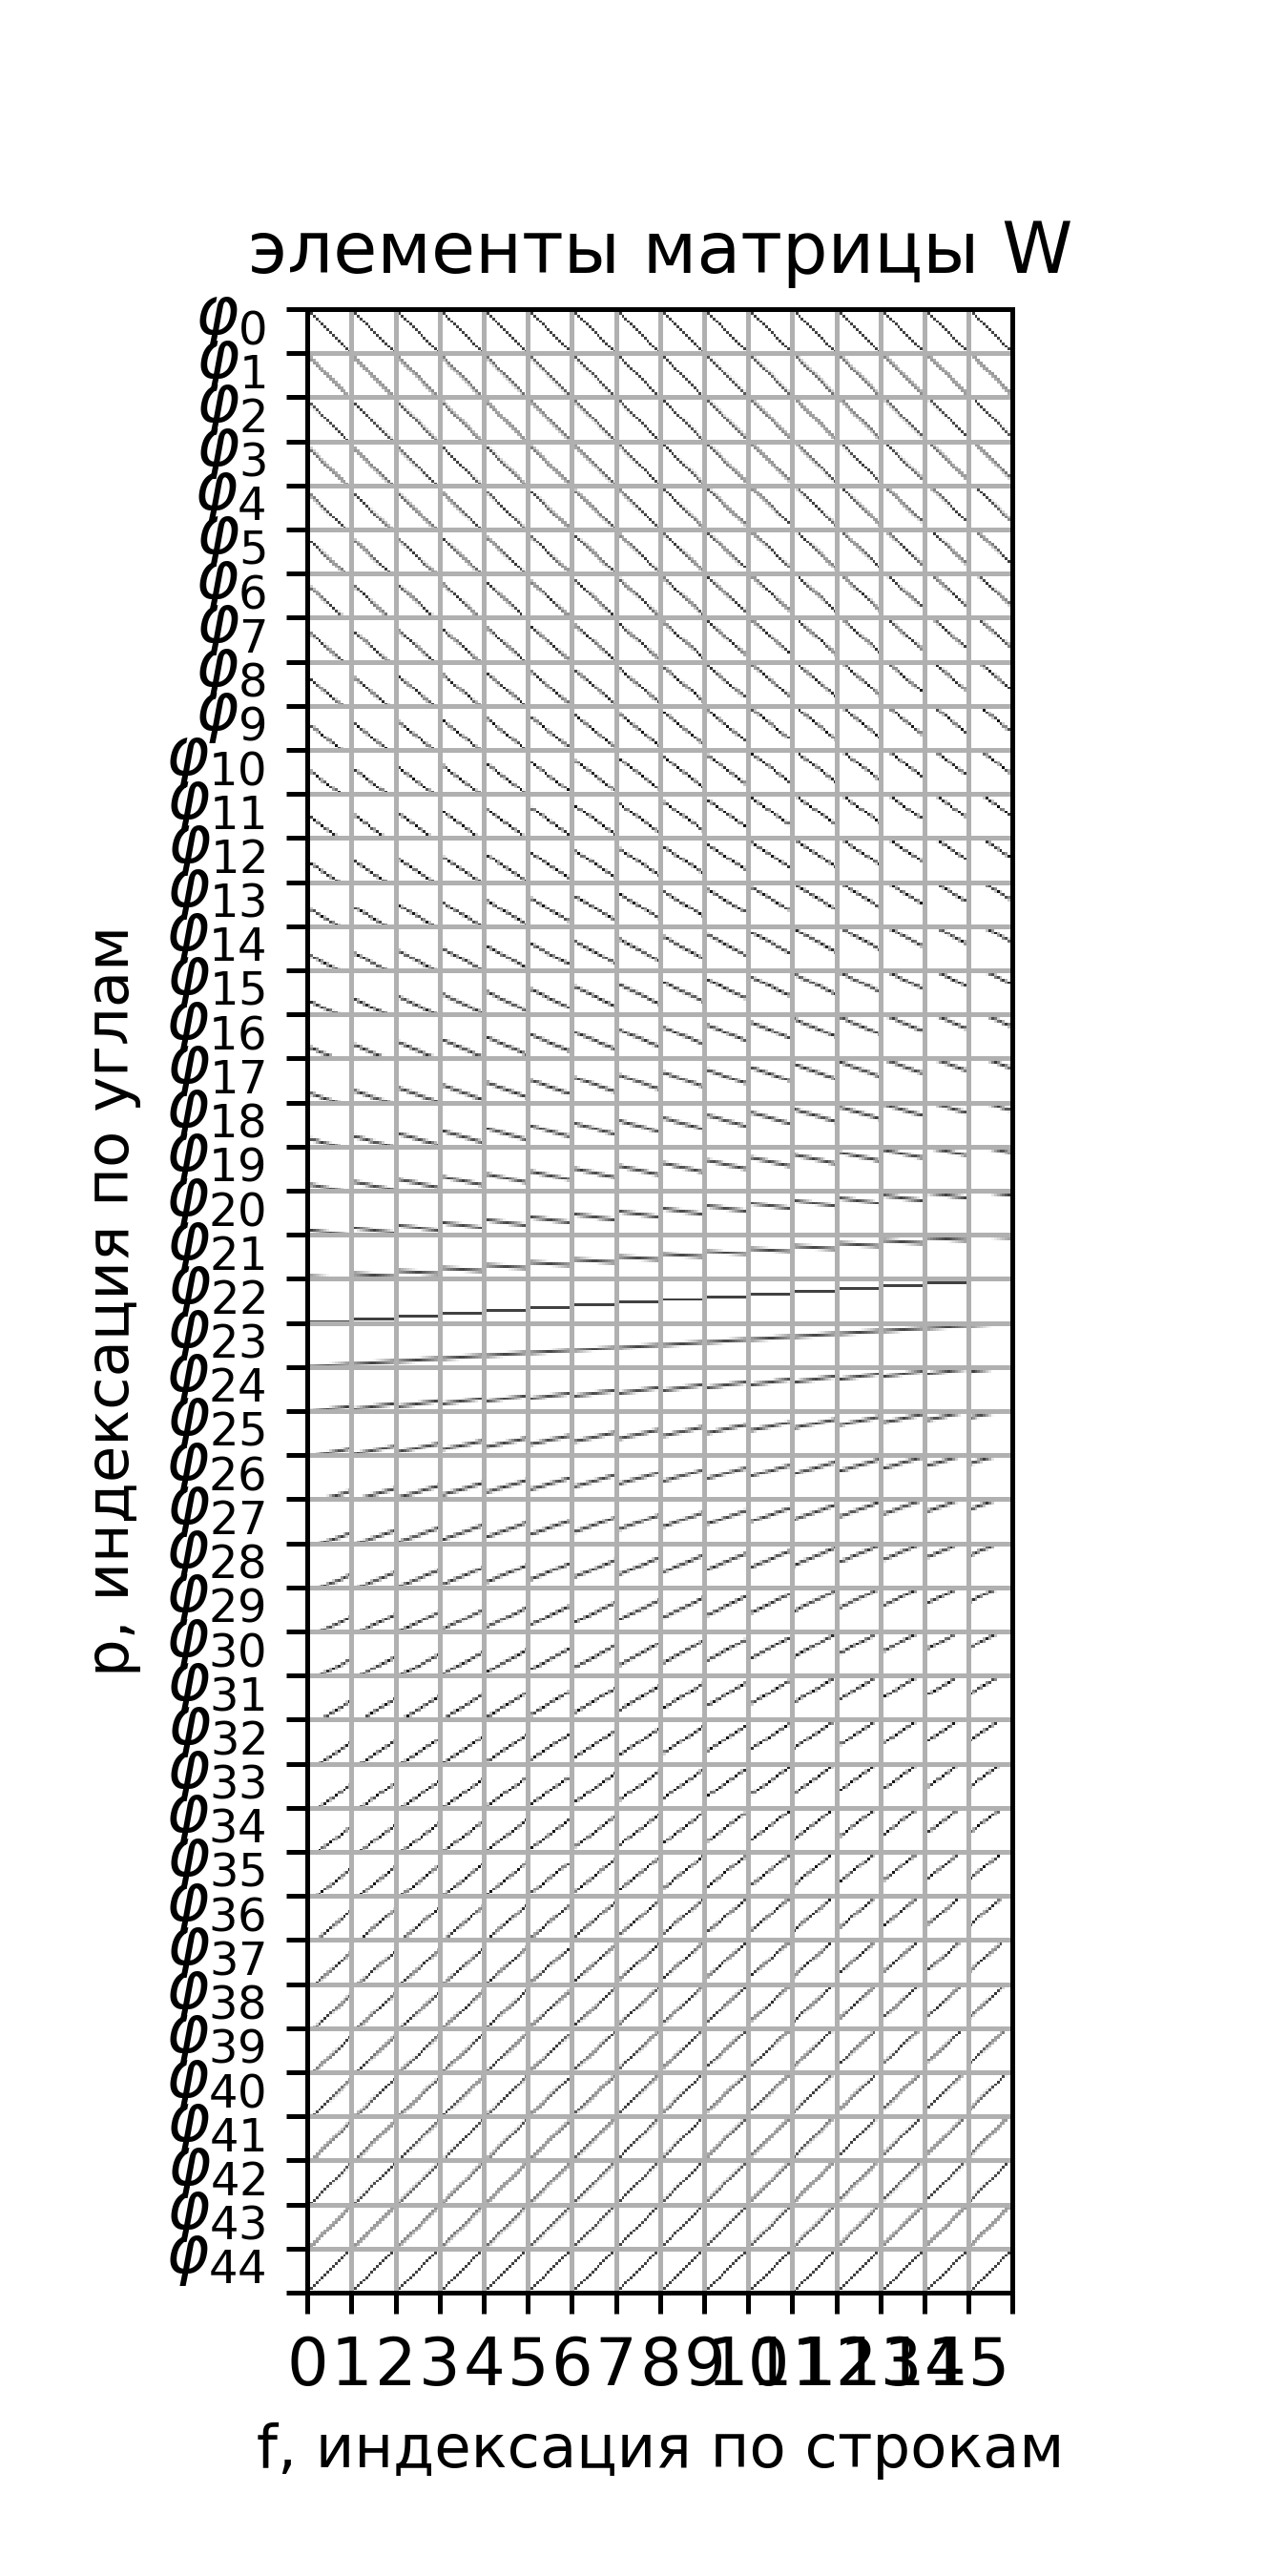
\includegraphics[width=0.25\textwidth]{../../Presentation/images/w_matrices/W_16_45_plot.png} \\
\small{$N = 10$, $N_\varphi = 10$} &
\small{$N = 10$, $N_\varphi = 35$} & 
\small{$N = 16$, $N_\varphi = 45$}
\end{tabular}
\caption{Примеры вычисленных матриц проекции W}
\label{fig:w_matrices}
\end{figure}

\section{Метод восстановления}

Формулировка задачи оптимизации, решение которой приводит к восстановленному изображению, приведена в \eqref{eq:quadprog_ineq}.
Это задача квадратичного программирования, хорошо известная и имеющая много готовых реализаций решающего ПО в популярных математических пакетах.
Для проверки подхода были использованы реализации пакета quadprog на языке Matlab \cite{coleman1996reflective} и пакета cvxopt для языка Python \cite{andersen2013cvxopt}.

В общем случае задача квадратичного программирования формулируется как 

\begin{equation}
  \label{eq:quadprog_general}
  \begin{cases}
  \frac 1 2 x^\mathrm{T}Px + q^\mathrm{T}x \rightarrow \min\limits_x & w.r.t \\
  Gx \preceq h \\
  Ax = b\,
  \end{cases}
\end{equation}

где $P$ --- симметричная положительно определнная матрица, а $Gx \preceq h$ означает поэлементное выполнение неравенства.
Одним из эффективных подходов к решению оптимизации такого вида являются методы внутренней точки.
На протяжении всей оптимизационной процедуры решение находится внутри области, удовлетворящей ограничениям.
Постепенно с приближением к оптимуму, решению позвояют приближаться ближе и ближе к границе, и, в конце концов, удовлетворяет необходимой точности решения задачи.
Это достигается за счет введения так называемых барьерных функций для ограничений-неравенств, вклад котрых ослабляется с ходом оптимизации.
А именно, для каждого неравенства $g_i^\mathrm{T}x \leq 0$ в целевую функцию добавляется аддитивный регуляризатор вида $\phi_i(x) = -\frac 1 t \log{\left(- g_i^\mathrm{T}x \right)}$.
Эти функции являются аппроксимациями индикаторной функции ограничений $I_i(x) = 0 \text{, если } g_i^\mathrm{T}x < 0 \text{, иначе} +\inf$.
Внутри области, удовлетворяющей ограничениям, функции являются гладкими.
Легко получить выражение для первой и второй производной барьерных функций:

\begin{equation} 
\label{eq:barrier_grads}
\begin{split}
  \nabla \phi_i(x) &= \frac 1 t \frac {g_i}{-g_i^\mathrm{T}x} \\
  \nabla^2 \phi_i(x) &= \frac 1 t \frac {g_i g_i^\mathrm{T}} {\left( g_i^\mathrm{T}x \right)^2}
\end{split}
\end{equation}

Задача \eqref{eq:quadprog_general} принимает вид

\begin{equation}
  \label{eq:quadprog_barrier}
  \begin{cases}
  \frac 1 2 x^\mathrm{T}Px + q^\mathrm{T}x + \frac 1 t \phi(x) \rightarrow \min\limits_x & w.r.t \\
  Ax = b\,
  \end{cases}
\end{equation}

где $\phi(x) = \sum_i \phi_i (x) = \sum_i {-\log{\left(- g_i^\mathrm{T}x \right)}}$ --- полная функция со всеми барьерными штрафами. 
Такая задача оптимизации решается методом Ньютона, а именно с помощью итеративной минимизации вида
%\begin{equation} \notag
\begin{gather}
\left(
  \begin{matrix}
  P + \frac 1 t \nabla^2 \phi_i(x) & A ^\mathrm{T} \\
  A & 0
  \end{matrix}
  \right)
  \left(
  \begin{matrix}
  \Delta x \\ \nu
  \end{matrix}
  \right)
  =
  \left(
  \begin{matrix}
  -x^\mathrm{T}P - q^\mathrm{T} - \frac 1 t \nabla \phi(x) \\ 0
  \end{matrix}
  \right),
\end{gather}
где за $\Delta x$ обозначен очередной инкремент итерации.
Далее метод барьерных функций представляет собой последовательное решение ``центрирующих'' задач вида \eqref{eq:quadprog_barrier} для растущей последовательности параметров $t, \mu t, \mu^2 t \dots$

Метод барьерных функций представляет собой общий инструментарий для рещения задач выпуклого программирования. 
В контексте сформулированной в \eqref{eq:quadprog_ineq} оптимизационной задачи получается ... \todo{вывести значения P, A G для томографической задачи}


\section{Результаты восстановления}
 \label{sect_2_resutls_qp_10x10}

\begin{figure}
  \centering
  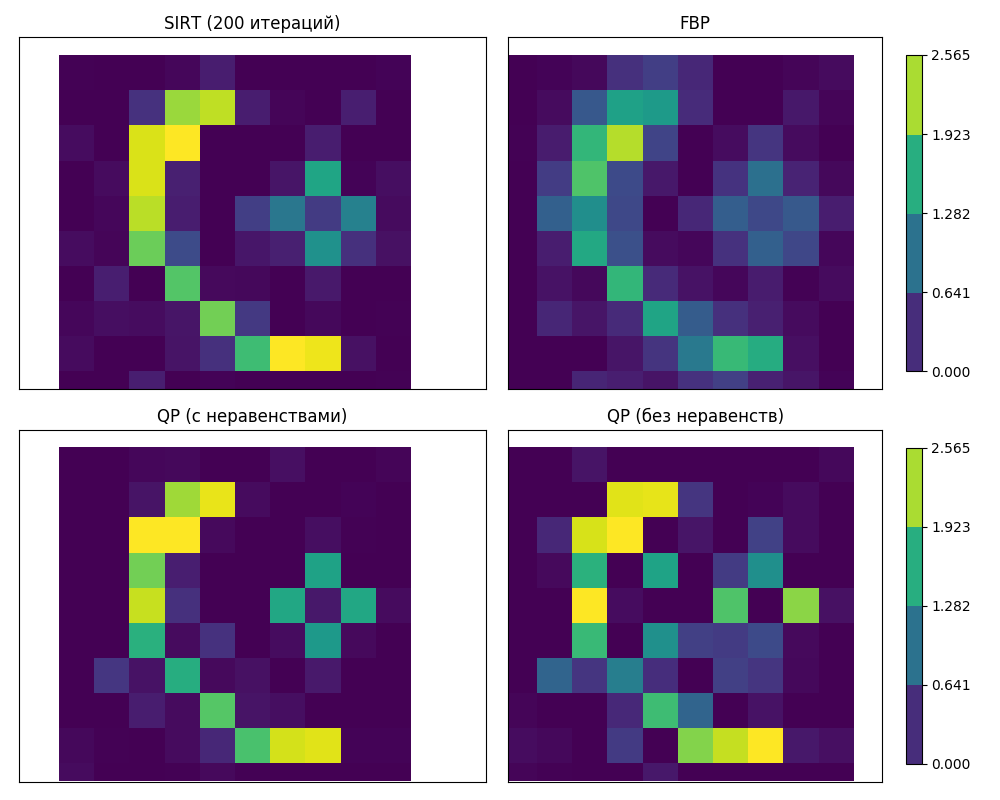
\includegraphics[width=0.7\textwidth]{part2_img/qp_foursome_10x10}
  \caption{Восстановление различными методами: a) SIRT, б) FBP, в) QP(с неравенствами), г) QP(без неравенств)}
  \label{im:quadprog}
\end{figure}

Для симуляции использовался фантом, изображенный на рисунке \ref{fig:qp_phantom_10by10}a).
На рисунке \ref{im:quadprog}a,б) представлено восстановление полученной синограммы методами SIRT и свертки и обратной проекции.
Целью данного подраздела является улучшение данного восстановения методом квадратичного программирования.
Результаты восстановления с помощью решения задачи \eqref{eq:quadprog_ineq} представлены на рисунке \ref{im:quadprog}в,г.
В одном случае использовалась информация, содержащаяся в неравенствах, в другом - все уравнения интерпретировались как равенства.
Интересным результатом является несовпадение результатов восстановлений а) и г).
Это можно объяснить различным количеством произведенных итераций, а так же незначительным раличием в форме итерации.
Для восстановления использовался метод \cite{quadprog_algo}.
Как видно из рисунка, квадратичное программирование с условиями неравенствами обеспечивает лучшее восстановление границ и интенсивностей исходного фантома. 
Значения интенсивностей на разных частях восстановленых фантомов приведены в таблице \ref{tb:quadprog_res}:

\begin{table}[h]
\label{tb:quadprog_res}
\centering
\begin{tabular}{ r| c| c| c| c| c|}
       & \ref{fig:qp_phantom_10by10}a & \ref{im:quadprog}a & \ref{im:quadprog}b & \ref{im:quadprog}c & \ref{im:quadprog}d \\ \hline
скобка & $250$                        & $226.07 \pm 27.64$ & $158.85 \pm 29.83$ & $216.79 \pm 34.79$ & $221.44 \pm 54.49$ \\ \hline
крест  & $160$                        & $124.42 \pm 16.95$ & $80.49 \pm 8.11$   & $148.44 \pm 8.50 $ & $148.76 \pm 62.65$ \\ \hline
\end{tabular}

\caption{Средние значения и стандартное отклонение интенсивностей в разных областях исследуемого фантома}
\end{table}

%FBP :  bracket: 158.85 +- 29.83 cross: 80.49 +- 8.11
%SIRT :  bracket: 226.07 +- 27.64 cross: 124.42 +- 16.95
%QP (с неравенствами) :  bracket: 216.79 +- 34.79 cross: 148.44 +- 8.50
%QP (без неравенств) :  bracket: 221.44 +- 54.49 cross: 148.76 +- 62.65


Так же можно заметить, что использование квадратичного программирование с ограничениями типа неравенство обеспечивет более близкие значения интенсивностей с меньшим значением отклонения.
На рисунках видно, что только метод на основе квадратичного программирования позволяет восстановить полость внутри области слабого поглощения.

\section{Продолжение результата на изображения б\'ольших размерностей}
Результаты, полученные в \ref{sect_2_resutls_qp_10x10} показывают, что необходимая для улучшения восстановления информация может быть выражена в виде неравенств, предложенных в модели.
Однако сам метод, использованный в главе, не подходит для практического применения на современных вычислителях.
Ранее отмечалось, что существующие реализации численных решений задач QP во-первых, требуют на вход вычисления матрицы $WW^{\mathrm T}$, а во-вторых явного обращения этой матрицы как гессиана минимизируемог функционала.

Поэтому основная задача далее --- найти способ воспользоваться информацией из неравенств, оставаясь при этом в рамках вычислительно эффективной процедуры восстановления.
Для этого предлагаются два подхода: метод барьерных функций и метод мягких ограничений. 
Оба этих подхода учитывают неравенства в виде аддитивных слогаемых в оптимизируемом функционале.
В методе мягких ограничений используются стандартные квадратичные штрафы, а методе барьерных функций --- логарифмические, определенные только в области, удовлетворяющей соответствующим неравенствам.

Для получения результатов и исследования обозначенных свойств предлагается фантом, указанный на рис. \ref{fig:qp_phantom_64by64}.
В отличие от примера из предыдущей секции, в данном случае используется физическая симуляция металлического (Au) включения в ткань зуба (Ca).
На рис.\ref{fig:qp_phantom_64by64}а) можно видеть очертания трех низкопоглощающих объектов из кальция (зубов), в среднем из которых присутствует золотое включение.
Параметры гамма-коррекции для иллюстрации подобраны таким образом, чтобы слабопоглощающее включение было контрастно видно на фоне яркого сильно поглощающего.
Для вычисления прямой проекции использовалось 90 проекционных углов, а так же пуассоновский шум.
Амплитуда шума совместно с интенсивностью излучения подбирались экспертом таким образом, чтобы сохранялся приемлимый уровень соотношения сигнал-шум.
Значения полных сечений рассеяния излучения на заданной энергии (45 КэВ) для выбранных материалов рассчитывалось с помощью программной библиотеки XRayLib \cite{xraylib}.
\todo{нужно ли упомянуть что ПО для симуляции и составления фантома а так же программная реализация метода мягких ограничений реализована Соколовым В.?}

\begin{figure}
    \centering
    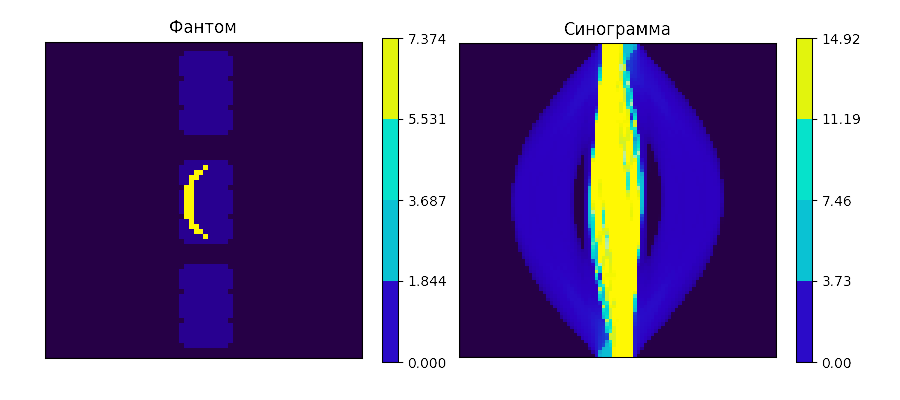
\includegraphics[width=0.9\textwidth]{part2_img/qp_input_64x64} \\
    а) \hspace{0.5\textwidth} б)
    \caption{а) Модельный фантом размера 64х64 пикселей. б) синограмма --- набор проекций данного фантома для 90 проекционных углов. К значениям интенсивностей применена гамма-коррекция для лучшего визуального представления }
    \label{fig:qp_phantom_64by64}
\end{figure}

Размер изображения 64х64 был выбран из соображений удобства разработки, чтобы иметь возможность производить большое количество тестовых прогонов алгоритмов восстановления на обычном ПК.
При этом методы, рассматриваемые в главе, могут быть применены для восстановления изображений и большего размера.


Обозначим за множество пикселей входной синограммы со значениями больше порога $\mathrm J = \{j | P_j \geq \delta \} \subseteq \{1 \dots n\}$, а так же введем диагональную матрицу-индикатор данного множества 
$$
K \in diag\left\{n \times n_\varphi\right\}; K_{jj} = 0 \text{, если\ } j \in \mathrm J \text{, иначе\ } 1
$$.
Каждому из неравенств, обозначающих вышедшие за порог значения интенсивностей в задаче \eqref{eq:quadprog_ineq} соответствует барьерная функция вида $\log{\sum_i f_{i} w_{ij} - \delta}$, если $j \in J$. 
А так же каждому пикселю восстанавливаемого изображения $i$ соответствует барьерная функция вида $\log{f_i}$.
Минимизируемый для решения задачи восстановления функционал принимает вид

\begin{equation}
\label{eq:barrier_method_goal}
  Q(f) = \Norm{K(P - Wf)}_2^2 - 
  \frac 1 t \left( 
    \sum_{j \in \mathrm J}{
      \log{\left(\sum_i {f_i w_{ij} - \delta} \right)}
    }
    +
    \sum_{i}{
      \log{f_i}
    }
  \right).
\end{equation}

Для решения оптимизационной задачи $Q(f) \rightarrow \min\limits_f$ применяется метод градиентного спуска.
Значения градиента для каждого из слагаемых в \eqref{eq:barrier_method_goal} рассчитываются следующим образом. 
Первая часть является обычной обратной проекцией ($BP(\cdot)$) невязки, с зануленными элементами, отвечающими $j \in \mathrm J$:
$$
\nabla_f \Norm{K(P - Wf)}_2^2 = 2 W ^ {\mathrm T} (K(Wf - P)) = 
  2 BP\left(K(Wf-P)\right).
$$

Для второго слагаемого, $\sum_j {\left(\log{\left(\sum_i {f_i w_{ij} - \delta} \right)}\right)}$, шаг градиентного спуска будет вычисляться как обратная проекция изображения, составленного из значений 
$$
\hat{h}_j = 
  \begin{cases}
    \left(\sum_i {f_i w_{ij}} - \delta \right)^{-1}, & \text{если}\ j \in \mathrm J \\
    0, & \text{иначе}
  \end{cases}.
$$
Напомним, что на протяжении итерационной процедуры выражение в знаменателе положительное, за $j$ обозначен индекс пикселя в пространстве измерений.
Итак,

$$
\nabla_f \sum_j {\left(
  \log{
    \left( \sum_i {f_i w_{ij}} - \delta \right)
  }
\right)} 
= BP(\hat{h}).
$$

Градиентом для третьего слагаемого будет изображение со значениями $\hat{u}_i = \frac 1 f_i$. Таким образом, шаг градиентного спуска для минимизации функционала $Q(f)$ будет иметь вид:

\begin{equation}
  \label{eq:barrier_method_gradstep}
  f^{\text{нов}} = f - \alpha \left(
    BP\left( K(Wf-P) \right) - 
    \frac 1 t BP(\hat{h}) - 
    \frac 1 t BP(\hat{u})
  \right),
\end{equation}

где за $\alpha$ обозначен параметр скорости градиентного спуска, или релаксационный параметр.
Настройка итерационного алгоритма, подобного (3) – сложная инженерная задача.
Необходима балансировка вкладов каждой из аддитивных составляющих градиента, чтобы они не выводили за пределы целевого множества.
Упростить эту настройку может использование операций проекции $f$ на целевое множество: после каждого обновления переменной  необходимо спроецировать ее на множества, задаваемые ограничениями $\sum_i {f_i w_{ij}} \geq \delta$ и $f_i \geq 0$.
Т.к. целевое множество и целевая функция – выпуклые, подобная регуляризация, помимо всего, ускоряет сходимость итерационной процедуры.
Чтобы сохранялась вычислительная стабильность итерационного процесса, проекция в реальности производится на множество, находящее во внутренности обозначенного целевого: $\sum_i {f_i w_{ij}} \geq \delta + \varepsilon$ и $f_i \geq \varepsilon$, где $\varepsilon$ --- некоторое маленькое число.
В описанных численных экспериментах использовалось значение $\frac {10^{-4}}{t}$.
Настройка производится с помощью подбора значений паметров метода:
\begin{itemize}
  \item шага градиентного спуска $\alpha$
  \item соотношения вкладов измерений и штрафов $\beta$
  \item начального значения параметра $t_0$
  \item допустимых отступов от границ ограничений $\varepsilon$
\end{itemize}

Проекции на множества ограничений, описываемые неравенствами, накладываемыми на восстанавливаемое изображение ($f_i \geq \varepsilon$), выполняются простым обрезанием значений: $f[f < 0] := 0$.
Однако чтобы спроецировать текущее решение на множества описываемые неравенствами относительно проекций, необходимо решить задачу, аналогичную задаче томографического восстановления.
Суть состоит в том, чтобы итеративно производить обратную проекцию по нарушающим ограничение измерениям, т.е. по таким лучам $j \in \mathrm J$, для которых выполняется $\sum_i f_i w_{ij} < \delta$.
Обозначим это множество за $\hat{\mathrm J}$.
Алгоритм проекции на множество ограничений в пространстве измерений представлен в алг. \ref{alg:hough_barrier_projection}.

\begin{algorithm}[H]

\vspace{0.5cm}
 % \Fn{\FnFeas{f}}{
 \Fn{\FnFeas{f}}{
 \KwData{текущее значение $f$, количество итераций $N$, допуск $\varepsilon$, скорость спуска $\alpha$}
 \KwResult{результат проекции $f$ на ограничения}
 $P := FP(f)$ \;\tcc*{вычисление прямой проекции}
 $\hat{\mathrm J} = \{j \in \mathrm J | P_j < \delta \}$\; \tcc*{множество нарушений ограничения}
 \For{i в интервале от 1 до $N$}{
  \If{$\hat{\mathrm J}$ --- пустое}
  {\KwRet $f$}
  \Else{
    $P[~\hat{\mathrm J}] := 0$\;
    $P[\hat{\mathrm J}] -= \delta + \varepsilon$\;
    $f := f - \alpha BP(P)$\;
  }
 }
 {\KwRet $f$}\;
 }
\vspace{0.5cm}

 \caption{Вычисление проекции решения на множество, описываемое ограничениями-неравенствами, наложенными на пространство измерений, в задаче \eqref{eq:quadprog_ineq}}
 \label{alg:hough_barrier_projection}
\end{algorithm}

Общий вид алгоритма восстановления методом барьерных функций представлен в \ref{alg:barrier_method}.
Результаты восстановленя модельного фантома рис. \ref{fig:qp_phantom_64by64}a) представлены на рисунке \ref{fig:qp_recres_64by64}

\begin{algorithm}[H]
\vspace{0.5cm}


 \KwData{измеренные проекции $P$, значение порога $\delta$, количество внешних итераций $N_b$,\\ начальное значение параметра $t_0$, скорость возрастания параметра $\beta$}

 \KwResult{восстановленное изображение $f$}
 инициализация $f$ значениями около 0 \;
 $f := \FnFeas(f)$ \;
 $t := t_0$ \;

 \For(\tcc*{барьерные итерации}){$i_b$ в интервале от 1 до $N_b$}{
% \For{$i_b$ в интервале от 1 до $N_b$}{
  \While(\tcc*{Поиск решения для барьерной итерации}){ошибка не на плато}{
  %\While{ошибка не на плато}{

  вычисление $FP(f)$, ошибки $Q(f)$ \;
  вычисление шага градиента \eqref{eq:barrier_method_gradstep}\;
  $f := \FnFeas(f)$\;
  }
  $t := t * \beta$ \;

 }

\vspace{0.5cm}
 \caption{Метод барьерных функций для задачи восстановления объектов с наличием сильнопоглощающих включений}
 \label{alg:barrier_method}
\end{algorithm}

Внешние итерации в алгоритме \ref{alg:barrier_method} по значениям параметра $t$ приближают задачу оптимизации к исходной.
Решение о переходе на следующую внешнюю итерацию принимается, когда найден некоторый минимум текущей задачи при зафиксированном значении параметра. 
В описанных в главе экспериментах использовалось следующее правило перехода к следующей итерации: если на протяжении 30 внутренних итераций не происходит существенного изменения суммарной ошибки $Q(f)$, значение параметра $t$ увеличивается в два раза.
Внешние итерации хорошо видны на графие ошибки (рис. \ref{fig:barrier_64by64_loss}) --- после увеличения параметра $t$ оптимизационная процедура вновь позволяет уменьшить ошибку шагами вдоль антиградиента. 


\begin{figure}
    \centering
    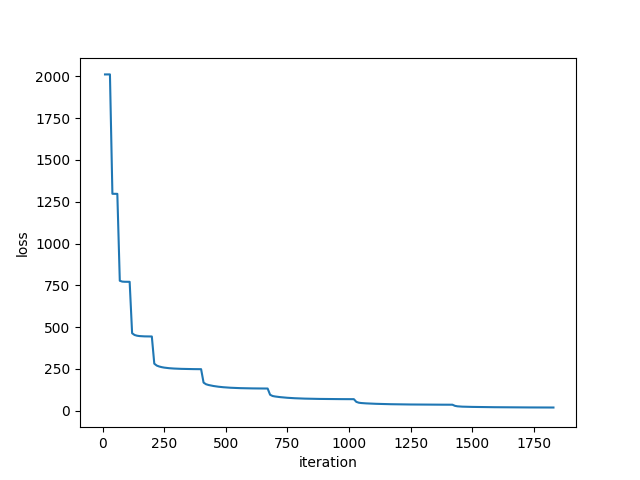
\includegraphics[width=0.7\textwidth]{part2_img/barrier_64by64_loss} \\
    \caption{ Зависимость ошибки $Q(f)$ от номера итерации. ``Ступеньки'' на графике соответствуют изменению параметра $t$}
    \label{fig:barrier_64by64_loss}
\end{figure}


\section{Мягкие ограничения на неравенства} \label{sect_2_2}

Другой метод восстановления, рассматриваемый в главе, отражает альтернативный способ приближения задачи квадратичного программирования \eqref{eq:quadprog_ineq} для возможности решения на изображениях большего размера.
Как и в случае с методом барьерных функций, ограничения-неравенства задачи переходят в аддитивные члены оптимизируемого функционала.
Однако, в отличие от метода барьерных функций, используются не логарифмические штрафы, а квадратичные:

\begin{equation}
  \label{eq:soft_ineq_goal}
  Q(f) =  \Norm{K(P - Wf)}_2^2 + \beta \Norm{(E-K)(\delta - Wf)_+}_2^2,
\end{equation}

где за $(\cdot)_+$ обозначена функция принимающая значение 0 в отрицательных значениях, и тождественная в положительных, то есть $(x)_+ = max(0, x)$.
Таким образом, целевая функция получает мягкий штраф только за нарушение неравенств.
Заметим, что слово ``мягкий'' здесь употребляется в том смысле, что, в отличие от метода квадратичного программирования со строгими неравенствами, здесь на решение не накладывается ограничений по их обязательному выполнению.
Результат восстановления может и не лежать в области, удовлетворяющей модельным органичениям, если это позволяет более точно соответствовать измерениям в остальных, не затемненных металлами, пикселях детектора.
Это позволяет методу быть более устойчивым относительно ошибок в измерениях: ошибочное затемненное значение будет непременно выполнено в методах QP и барьерных функций, так как решение ищется строго в допустимом множестве, в то время как в методе мягких ограничений штрафуется лишь грубое нарушение неравенства.
Соотношение вкладов томографической невязки и мягкого ограничения регулируется параметром $\beta$.
Аналогичного поведения в задаче QP можно добиться, введя дополнительные переменные нежесткотси $\xi_s \geq 0, \zeta_i \geq 0 $ (slackness) и решая задачу большей размерности:

$$
  \begin{cases}
  \Norm{P^{\textup{изм.}} - Wf}_2^2 + C_\xi \sum_s \xi_s + C_\zeta \sum_i \zeta_i \rightarrow \min\limits_{f, \xi_s, \zeta_i} & w.r.t \\
  \sum_i f_{i} w_{ij} > \delta - \xi_s, & \mbox{если } P^{\textup{изм.}}_j = \delta, \\ 
  f_{i} \geq -\zeta_i, \\
  \xi_s \geq 0, \zeta_i \geq 0
  \end{cases}.
$$

Здесь за соотношение вкладов нежесткости и целевой функции отвечает аналогичная переменная, традиционно обозначаемая за $С$.

Для наглядности на рис. \ref{fig:log_vs_l2} приведен вид функций штрафа для обоих рассматриваемых методов.

\begin{figure}
    \centering
    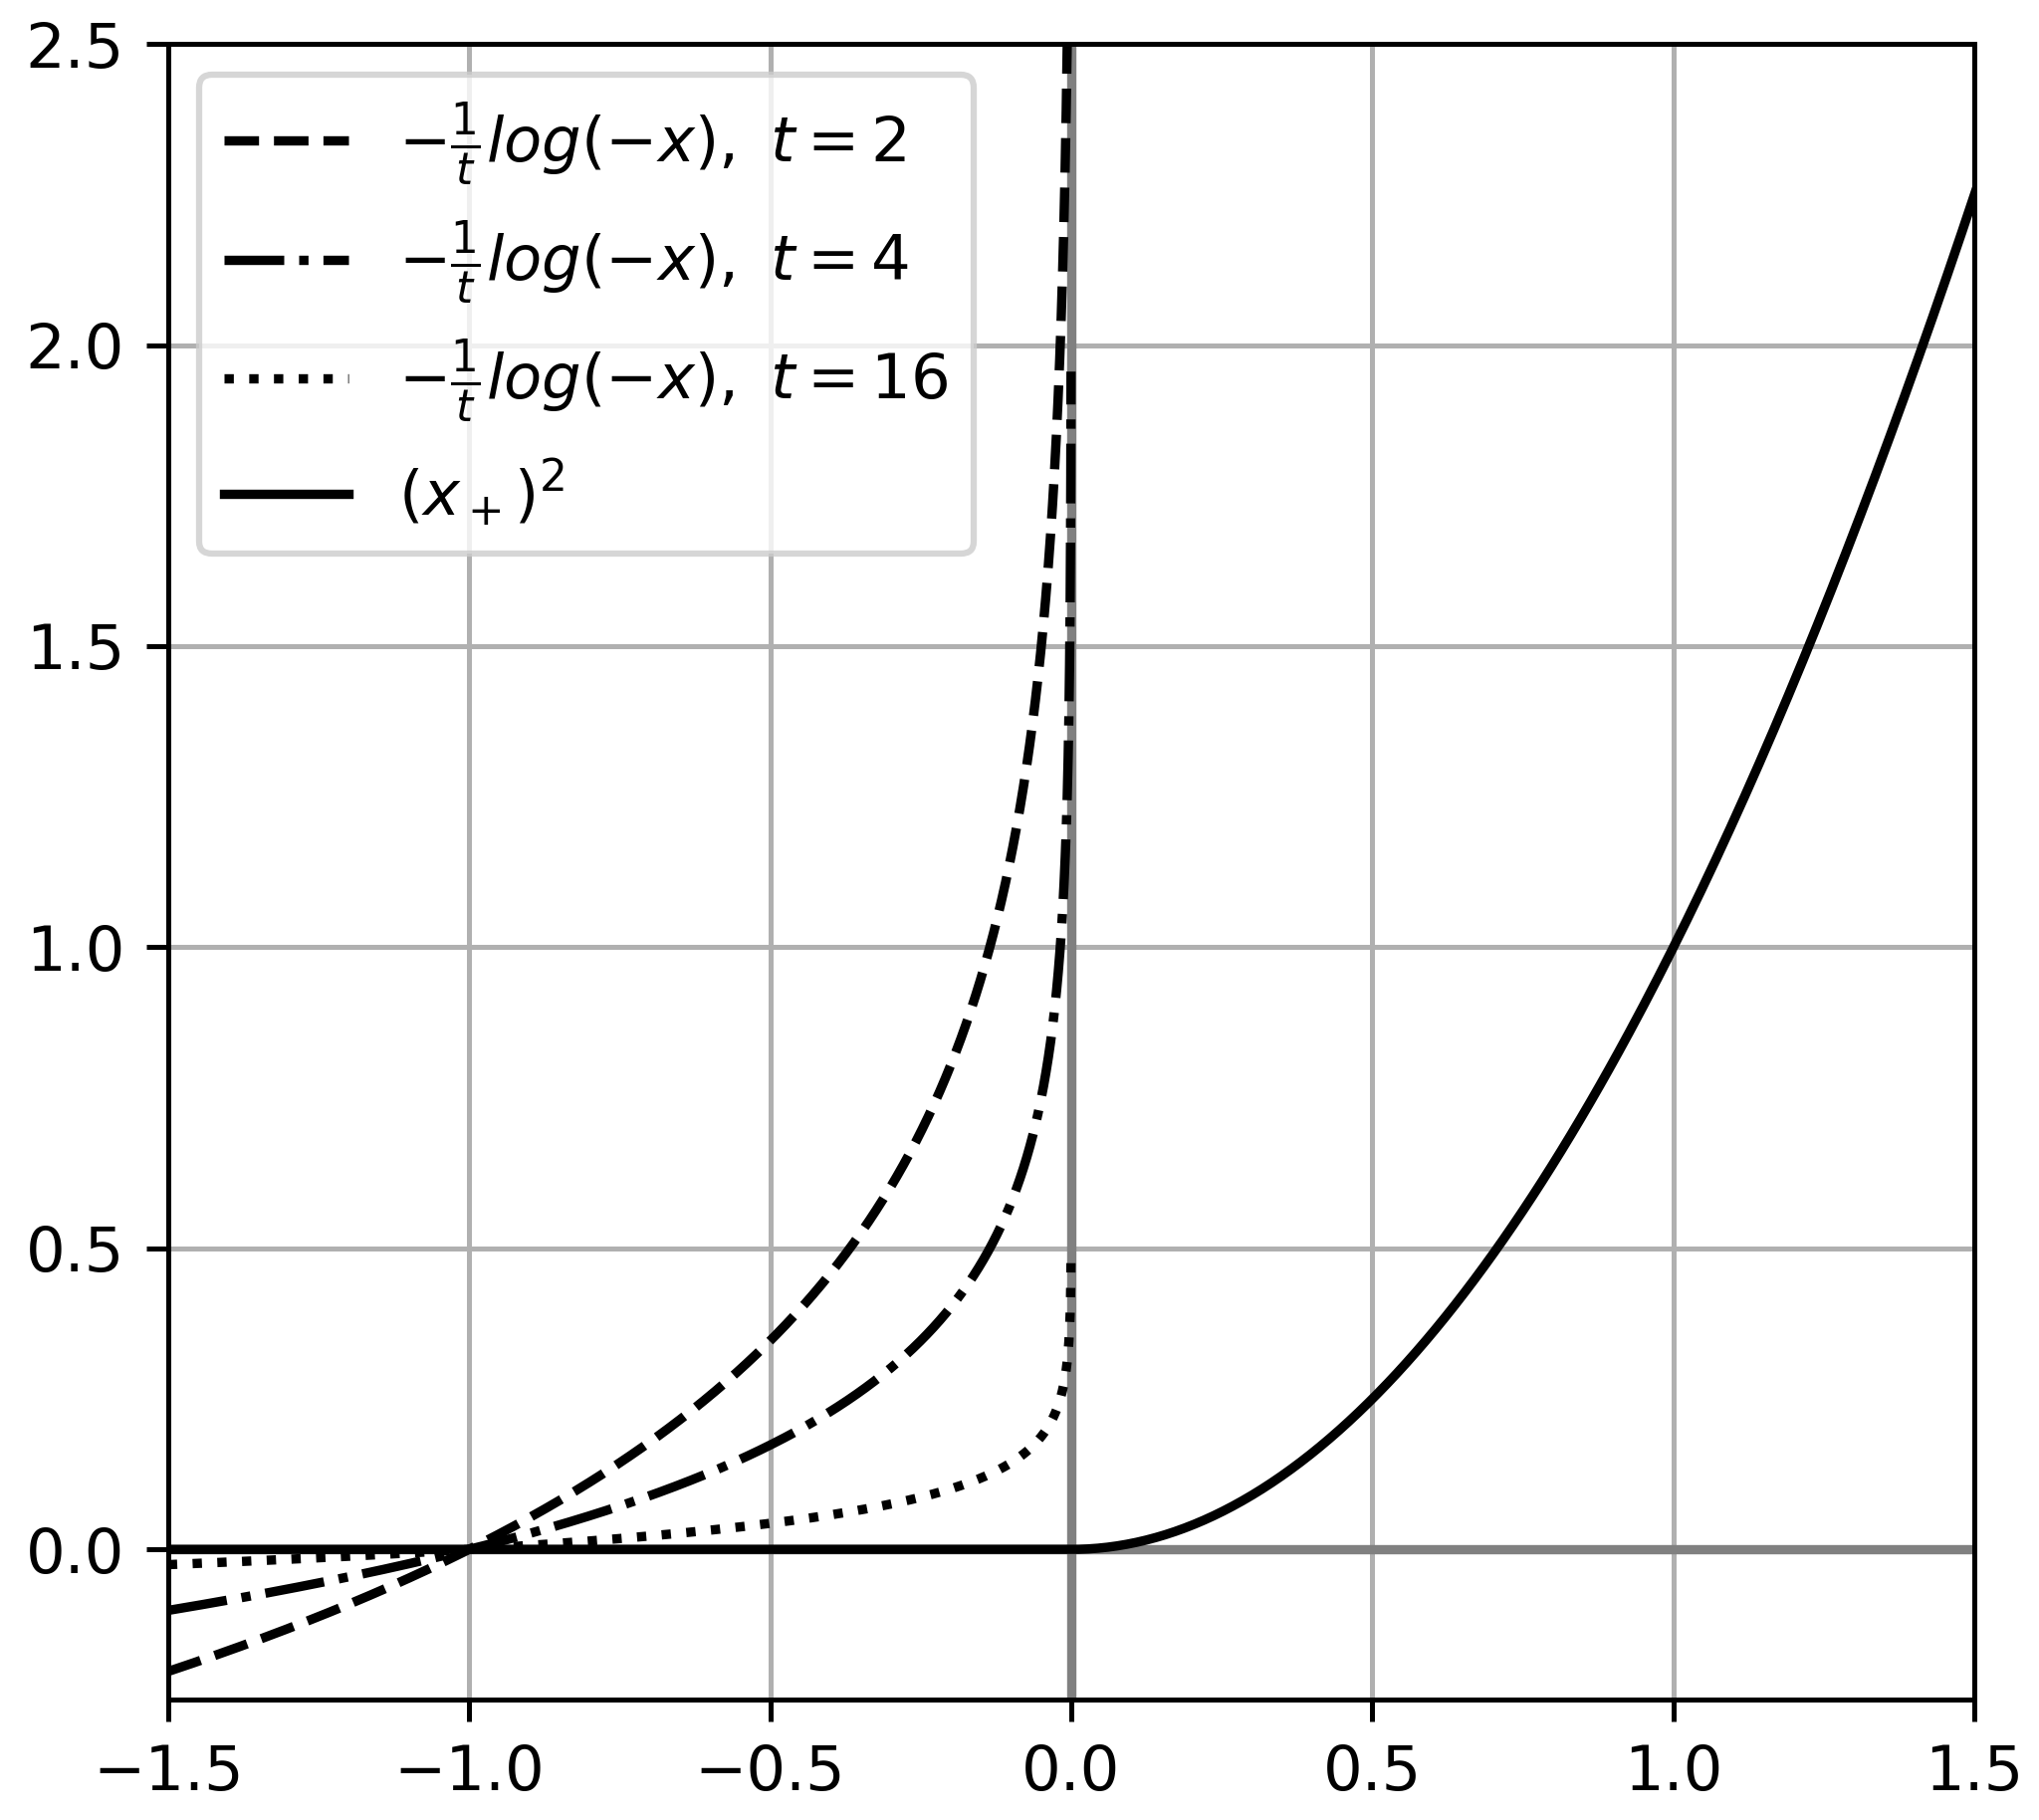
\includegraphics[width=0.65\textwidth]{part2_img/log_vs_l2} \\
    \caption{Сравнение вида функций штрафов вместо неравенств в методе барьерных функций и в методе мягких ограничений}
    \label{fig:log_vs_l2}
\end{figure}

Оптимизация функции \eqref{eq:soft_ineq_goal} выполняется с помощью метода сопряженных градиентов.
Способ вычисления градиентов для слогаемых целевой функции легко выражается тривиальным образом.
Для первого слагаемого он аналогичен \eqref{eq:barrier_method_goal}.
Второе слогаемое дает следующий вклад в шаг итерации:
$$
\nabla_f \Norm{(E-K)(\delta - Wf)_+}_2^2 = 2 (E-K) BP\left((Wf - delta)\right).
$$


\section{Результаты восстановления на симуляции}
Для исследования работы алгоритмов и сравнения результатов восстановления был разработан комплекс программ, реализующий симуляцию томографических измерений, алгоритмы восстановления, описанные в главе, сравнение и визуализацию результатов.
Программный комплекс реализован на языке Python, с использованием библиотек для научных вычислений Scipy \cite{scipy} и эффективных вычислительных томографических примитивов ASTRA \cite{van2015astra}.
Разработанный программный комплекс с открытым программным кодом доступен в github \cite{whitomo}.

На рис. \ref{fig:qp_recres_64by64} представлены фантом и  результаты его восстановления методами FBP, барьерных функций, мягких ограничений. 
Напомним, что исследуемый объект состоит из трех областей из кальция, с золотым включением в средней области.
Для лучшего визуального восприятия изображения были подвергнуты одинаковым преобразованиям контраста и гамма-коррекции.
На восстановленных картинах явно видно наличие артефактов, выраженных в ложном наличии полос из вещества, похожего на Ca по значению коэффициента ослабления.
Восстановление методом FBP не позволяет сохранить границы областей низкого поглощения, форма и поглощающая способность металлического включения так же неправильная.
Метод мягких ограничений дает сильно сглаженную картину, с размытием границ областей низкого поглощения, но более четкой формой металлического включения.
Наконец, метод барьерных функций позволяет оценить форму двух низкопоглощающих областей, не содержащих включения, а так же верно восстанавливает интенсивность металлического включения, т.е. эту картину можно использовать для анализа состава обработанного образца.
Количестванные оценки качества восстановлений приведены в таблице \ref{tb:res_64by64}.
Видно, что только методу барьерных функций удалось правильно восстановить поглощающую способность металлического включения.
Большой разброс в значениях обусловлен наличием артефактов восстановления.
Процент правильно определнных поглощающих способностей рассчитывался по попаданию интенсивности восстановления в окрестность правильных значений: для фона окрестность была $\pm 0.05$, для зуба --- $\pm 0.95$, для металла --- $\pm 7.5$.

\begin{table}[]
\label{tb:res_64by64}
\centering
\begin{tabular}{|l|l|l|l|l|l|}
\hline
& & фантом & FBP & \begin{tabular}[c]{@{}l@{}}Метод\\ барьерных\\ функций\end{tabular} & \begin{tabular}[c]{@{}l@{}}Метод\\ мягких\\ ограничений\end{tabular} \\ \hline
\multirow{2}{*}{фон} & $\mu \pm \sigma$ & 0      & $0.026 \pm 0.072$ & $0.03 \pm 0.08$                                                     & $0.033 \pm 0.086$                                                       \\ \cline{2-2} \cline{4-6} 
& \% верных        &        & \textbf{88.3 \%}  & 83.1 \%                                                             & 85.2 \%                                                                 \\ \hline
\multirow{2}{*}{зуб(Ca)}                                               & $\mu \pm \sigma$ & 0.104  & $0.245 \pm 0.436$ & $0.462 \pm 1.684$                                                   & $0.311 \pm 0.533$                                                       \\ \cline{2-2} \cline{4-6} 
& \% верных        &        & 91.5 \%           & \textbf{92.9 \%}                                                    & 86.3 \%                                                                 \\ \hline
\multirow{2}{*}{\begin{tabular}[c]{@{}l@{}}металл\\ (Au)\end{tabular}} & $\mu \pm \sigma$ & 9.218  & $2.190 \pm 0.638$ & $9.415 \pm 5.355$                                                   & $1.726 \pm 0.152$                                                       \\ \cline{2-2} \cline{4-6} 
& \% верных        &        & 80.7 \%           & \textbf{100 \%}                                                     & 46.1 \%                                                                 \\ \hline
\end{tabular}
\\


\caption{Средние значения и стандартное отклонение интенсивностей в разных областях исследуемого фантома, а так же процент верно восстановленных пикселей}

\end{table}

\todo{таблица параметров, график оптимизации и количество итераций}


\begin{figure}
    \centering
    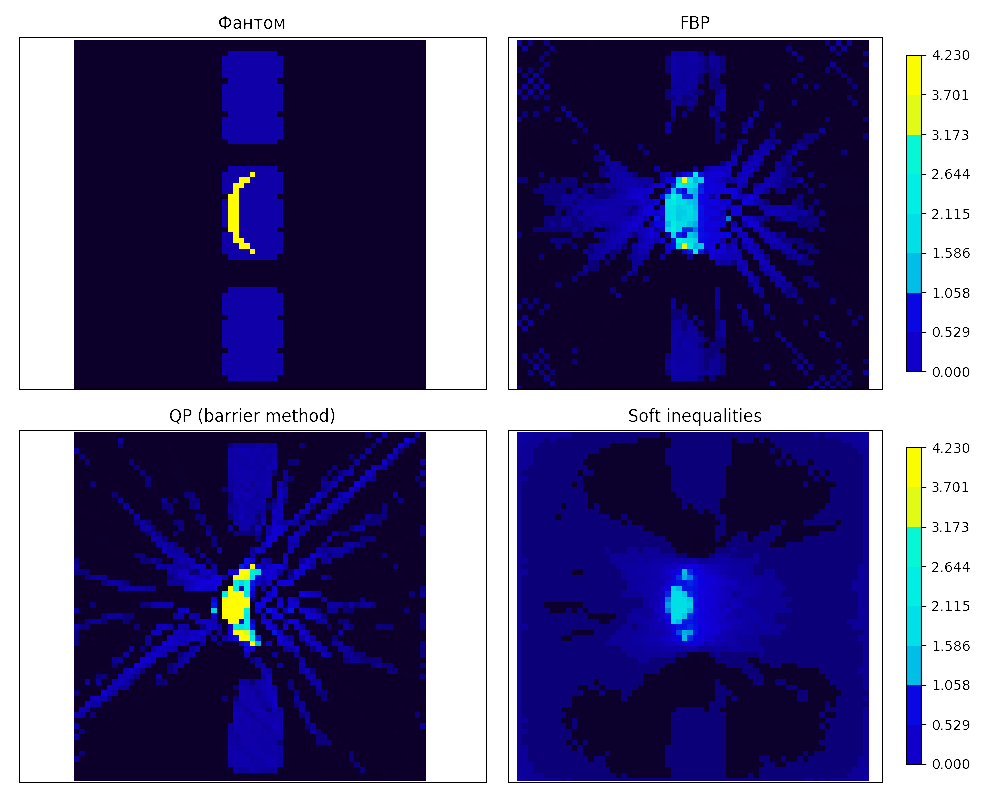
\includegraphics[width=0.9\textwidth]{part2_img/qp_foursome} \\
    \caption{а) фантом. б) результат восстановления методом FBP. в) Результат восстановления методом барьерных функций. г) результат восстановления методом мягких ограничений.}
    \label{fig:qp_recres_64by64}
\end{figure}

\begin{comment}

In this paper, we improve the results achieved in \cite{chukalinaway}. First, we provide a robust to noise and admissible to efficient optimization methods way to express the inequalities introduced in \cite{chukalinaway}. Second, we evaluate the method's performance on a simulated phantom data. The phantom data was simulated to remind a teeth with a metal object. And finally we evaluate the gain we get using the information in the inequalities against not using it at all.

The sections are organized as follows. Section \ref{s-approach} outlines the detail our approach to solve the problem. In Section \ref{s-phantom} the simulated phantom is presented. The obtained results are discussed in Section \ref{s-results}. Section \ref{s-conclusion} then concludes the whole paper.

% \section{Описание подхода}
\label{s-approach}
Let us denote the distribution of the attenuation coefficient in the reconstructed volume with $x \in \mathbb{R}^m$. The $p \in \mathbb{R}^n$ denotes the projection data detected during a scan. According to Beer-Lambert law the energy, detected at the detector cell, corresponding to $i$-th ray is expressed by the formula $p_i = I_0 * \exp(-a_i^T x)$, where $I_0$ is the source intensity, and $a_i$ is the row of the projection matrix $A$ corresponding to the $i$-th ray. A standard approach to find $x$ from the projection data is to take a logarithm and solve the linear system of equations: $Ax = r$, where
$r_i = \log(I_0) - \log(p_i)$. A standard way to get robust to noise reconstruction here is to use linear least squares:
\begin{equation} \label{eq:lls}
  \Norm{Ax - r}^2 \to \min\limits_{x}.
\end{equation}

Metal streak artifacts are caused mainly by photon starvation and noise. Mathematically it corresponds to the rays where $p_i$ is small or even zero. In latter case the logarithm is not defined and the simples way is just to ignore those rays solving instead of \eqref{eq:lls}:
\begin{equation}
  \label{eq:mask-lls}
  \Norm{P(Ax - r)}^2 \to \min\limits_{x},
\end{equation}
where matrix $P$ takes only those coordinates of a vector, at which $p_i \neq 0$. More precisely,
$$
P_{i,j} = \begin{cases}
  1, \quad\text{if $i = j$ and $p_i > 0$} \\
  0, \quad\text{otherwise}
  \end{cases}.
$$

It was suggested in \cite{chukalinaway} that even such problematic rays provide us with some information, namely that the weighted sum along such a ray has lower bound $a_i^T x > B$, for some suitable value of $B$ (for example, $B = \log I_0$), and we can use this information in a form of linear inequality constraints, solving the linear system with linear least squares approach:
\begin{equation}
  ||P(Ax - r)||^2 \to \min\limits_x, \quad\textrm{s.t. }  QAx \ge B,
\end{equation}
where $Q$ takes only those coordinates of a vector at which $p_i = 0$, opposite to the matrix $P$. Basically, $Q = E - P$, where $E$ is identity matrix.

This constraints being mathematically correct, are tight and are not robust against the noise in the projection data. Instead of tight constraints we propuse to use a soft version provided with a quadratic penalty method \cite{nocedal2006numerical} instead:
\begin{equation}
  \label{eq:soft-ineq}
  ||P(Ax - r)||^2 + \alpha ||[QAx - B]^-||^2 \to \min\limits_x,
\end{equation}
where $[y]^- = \min\{0, y\}$.

This functional provides a soft way to enforce the inequalities on the variables, but also allows to handle noise effects more smoothly. We can regulate the effect of that smoothing by manipulating $\alpha$: the greater $\alpha$ is tighter the effect of inequalities is.

The objective function \eqref{eq:soft-ineq} is convex and differentiable. We can effectively minimize it with Conjugate Gratient method (we used the implementation of this method, provided by the Python package \cite{scipy}). To speed-up computation of forward and backward tomographic projection operators we used ASTRA Toolbox \cite{palenstijn2011performance, van2015astra} which performs efficient evaluation of such operators on GPU.
\begin{figure}[h]
  \centering
  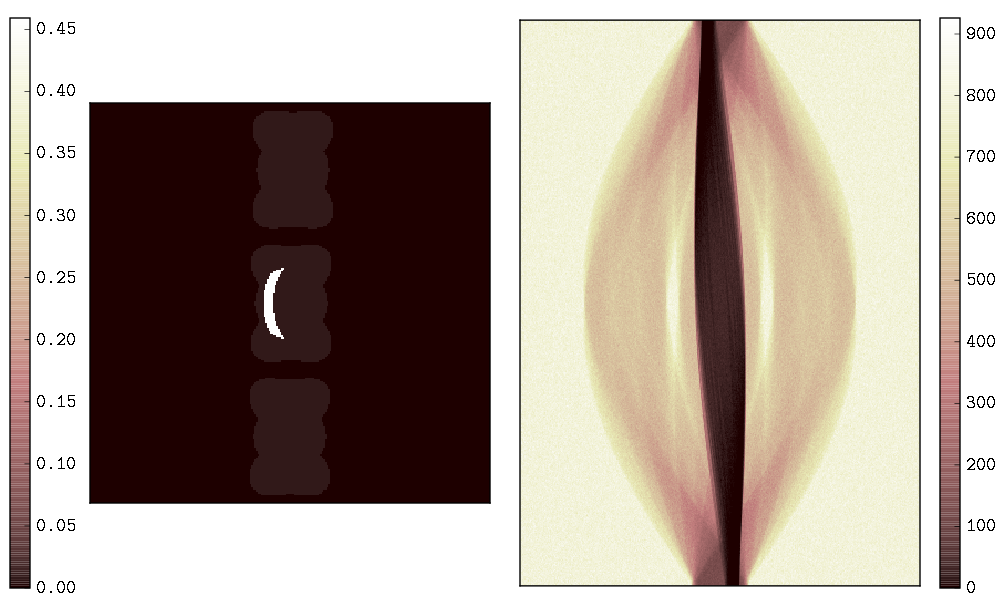
\includegraphics[scale=0.45]{part2_img/phantom-and-projection}
  \caption{The phantom (left) and its projection at $I_0 = 10^3$ photons (right).}
  \label{phantom-and-projection}
\end{figure}

\section{Описание образца}
\label{s-phantom}
To simulate the sinogram in $55$keV monochromatic mode we used a phantom imitating three teeth. Middle tooth contains titanium include imitating an implant (fig. \ref{phantom-and-projection}, left image). Pixel size is $0.005$cm. 2D field view size is $256 \times 256$ pixels. We used the XRayLib library \cite{brunetti2004library, schoonjans2011xraylib} to calculate the X-ray attenuation in each pixel for chosen energy. The sinogram (fig. \ref{phantom-and-projection}, right image) was calculated in a parallel scheme. We used $512$ rotation angles uniformly distributed in the interval $[0, \pi)$. The number of the detector cells is $362$, so that the diagonal of the phantom is projected on the detector without loosing any information. Such geometry choice allowed us to ignore the uniqueness of the solution issues which are related to the null-space of the projection operator and are ususally dealt with some sort of regularization techniques.

\section{Результаты}
\label{s-results}
To study the proposed approach we generated projections for different source intensities and draw several samples of Poisson noise at each source intensity.

For each projection we reconstructed the volume using Missing Data Least Squares \eqref{eq:mask-lls} and proposed Soft Inequalities Least Squares \eqref{eq:soft-ineq} approaches. The value of $\alpha$ was chosen to be equal to $50$.. The reconstructed volume was then compared to the original phantom and Mean Square Error was compute for such a pair.

In the figure \ref{sample} we can see an example of such reconstructions. In absence of the information encoded in the inequalities the metal artifacts are presented and there is a strong shadow in the cental tooth, while in the left image, reconstructed with Soft Inequalities approach those artifacts are significantly reduced.
\begin{figure}
  \centering
  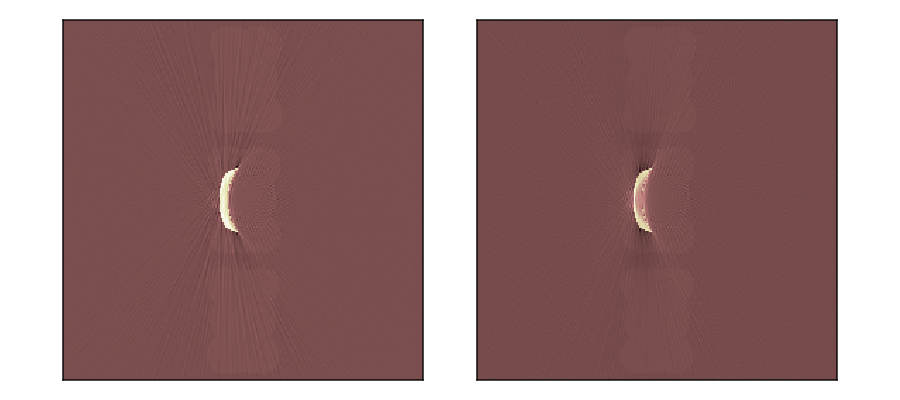
\includegraphics[scale=0.5]{part2_img/sample}
  \caption{Example of reconstruction with Soft Inequalities method (left)
    and Missing Data method (right).}
  \label{sample}
\end{figure}
In the figure \ref{error-plot} we can see the plot of MSE averaged over all the samples of noise for each noise level. The inequalities provide an improvement over ignoring such data at all noise levels.
\begin{figure}
  \centering
  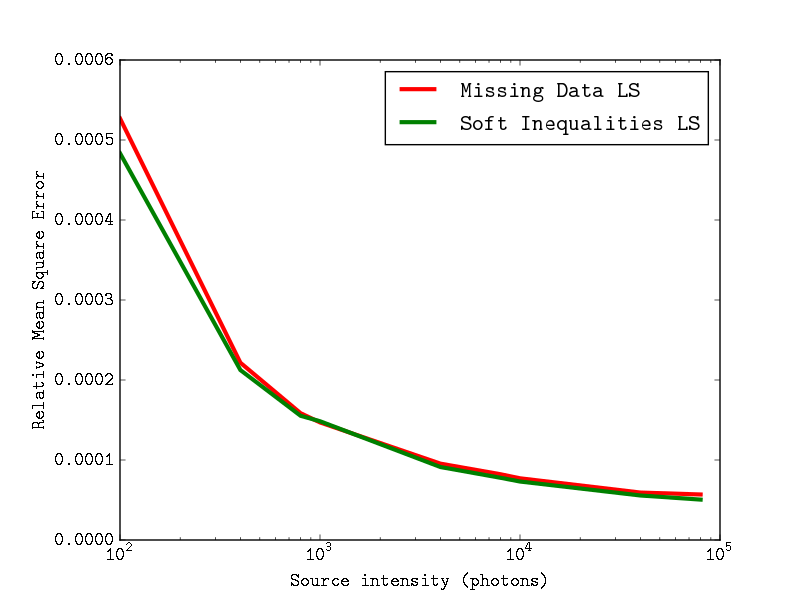
\includegraphics[scale=0.5]{part2_img/error-plot}
  \caption{The MSE value with respect to noise level.}
  \label{error-plot}
\end{figure}

\section{Выводы}
\label{s-conclusion}

Experiments shows that the information encoded in the inequalites, introduced in \cite{chukalinaway} carries a significant information which can be used to reduce metal-like artifacts in the reconstructions. We proposed a robust way to use this information in form of panaltized objective function. The proposed functional is suitable to be minimized with an efficient numerical algorithms enabling the approach to work on mid- and large-sized data. Proved to work, the method next should be deeper with respect to sensitivity to $\alpha$ and compared against the other approaches mentioned in the introduction. It is also seems possible to leave the penalty encoding the inequality constraints, replacing the least squares functional with more statistically suitable (for example, Poisson log-likelihood, used in MLEM) data fit functional.

\end{comment}

\subsection{параметры моделирования и восстановления} \label{sect_2_3}
Параметры моделирования:
\begin{itemize}
  \item размером фантома (size, 65, 256),
  \item количеством углов проекции (n\_angles, 90, 512), 
  \item интенсивность пучка (i0, 1000)
  \item энергия пучка (45 кэв)
  \item форма фантома (три зуба и имплант-бумеранг)
  \item материалы фантома и импланта (Ca, Au)
  \item наличие импланта (в наличии)
  \item размер пикселя (0.05)
  \item наличием шума при прокеции, распределением шума (есть пуассоновский шум)
\end{itemize}

Параметры восстановления:
\begin{itemize}
  \item итераций 200 (где-то 300)
  \item $\alpha$ 30 и 300
\end{itemize}

\section{Описание экспериментальных измерений}
Для проверки работы алгоритма на реальных экспериментальных данных были проведены томографические измерения на лабораторном микротомографе ФНИЦ ``Кристаллография и фотоника'' ИК РАН.
Измерения проводились на излучении, полученном c помощью рентгеновской электронной трубки с молибденовым (Mo) анодом.
Экспериментальный образец, использованный для измерений, представлял собой молочный зуб (рис. \ref{fig:sino_zub}в,г).
В зубе было сделано отверстие, в которое было помещено сильно поглощающее алюминиевое включение.
Спектр испускания анода, а так же спектральные функции поглощения для материалов зуба (Ca) и включения (Pb) представлены на рис. \ref{fig:zub_spectre}.

\begin{figure}
    \centering
    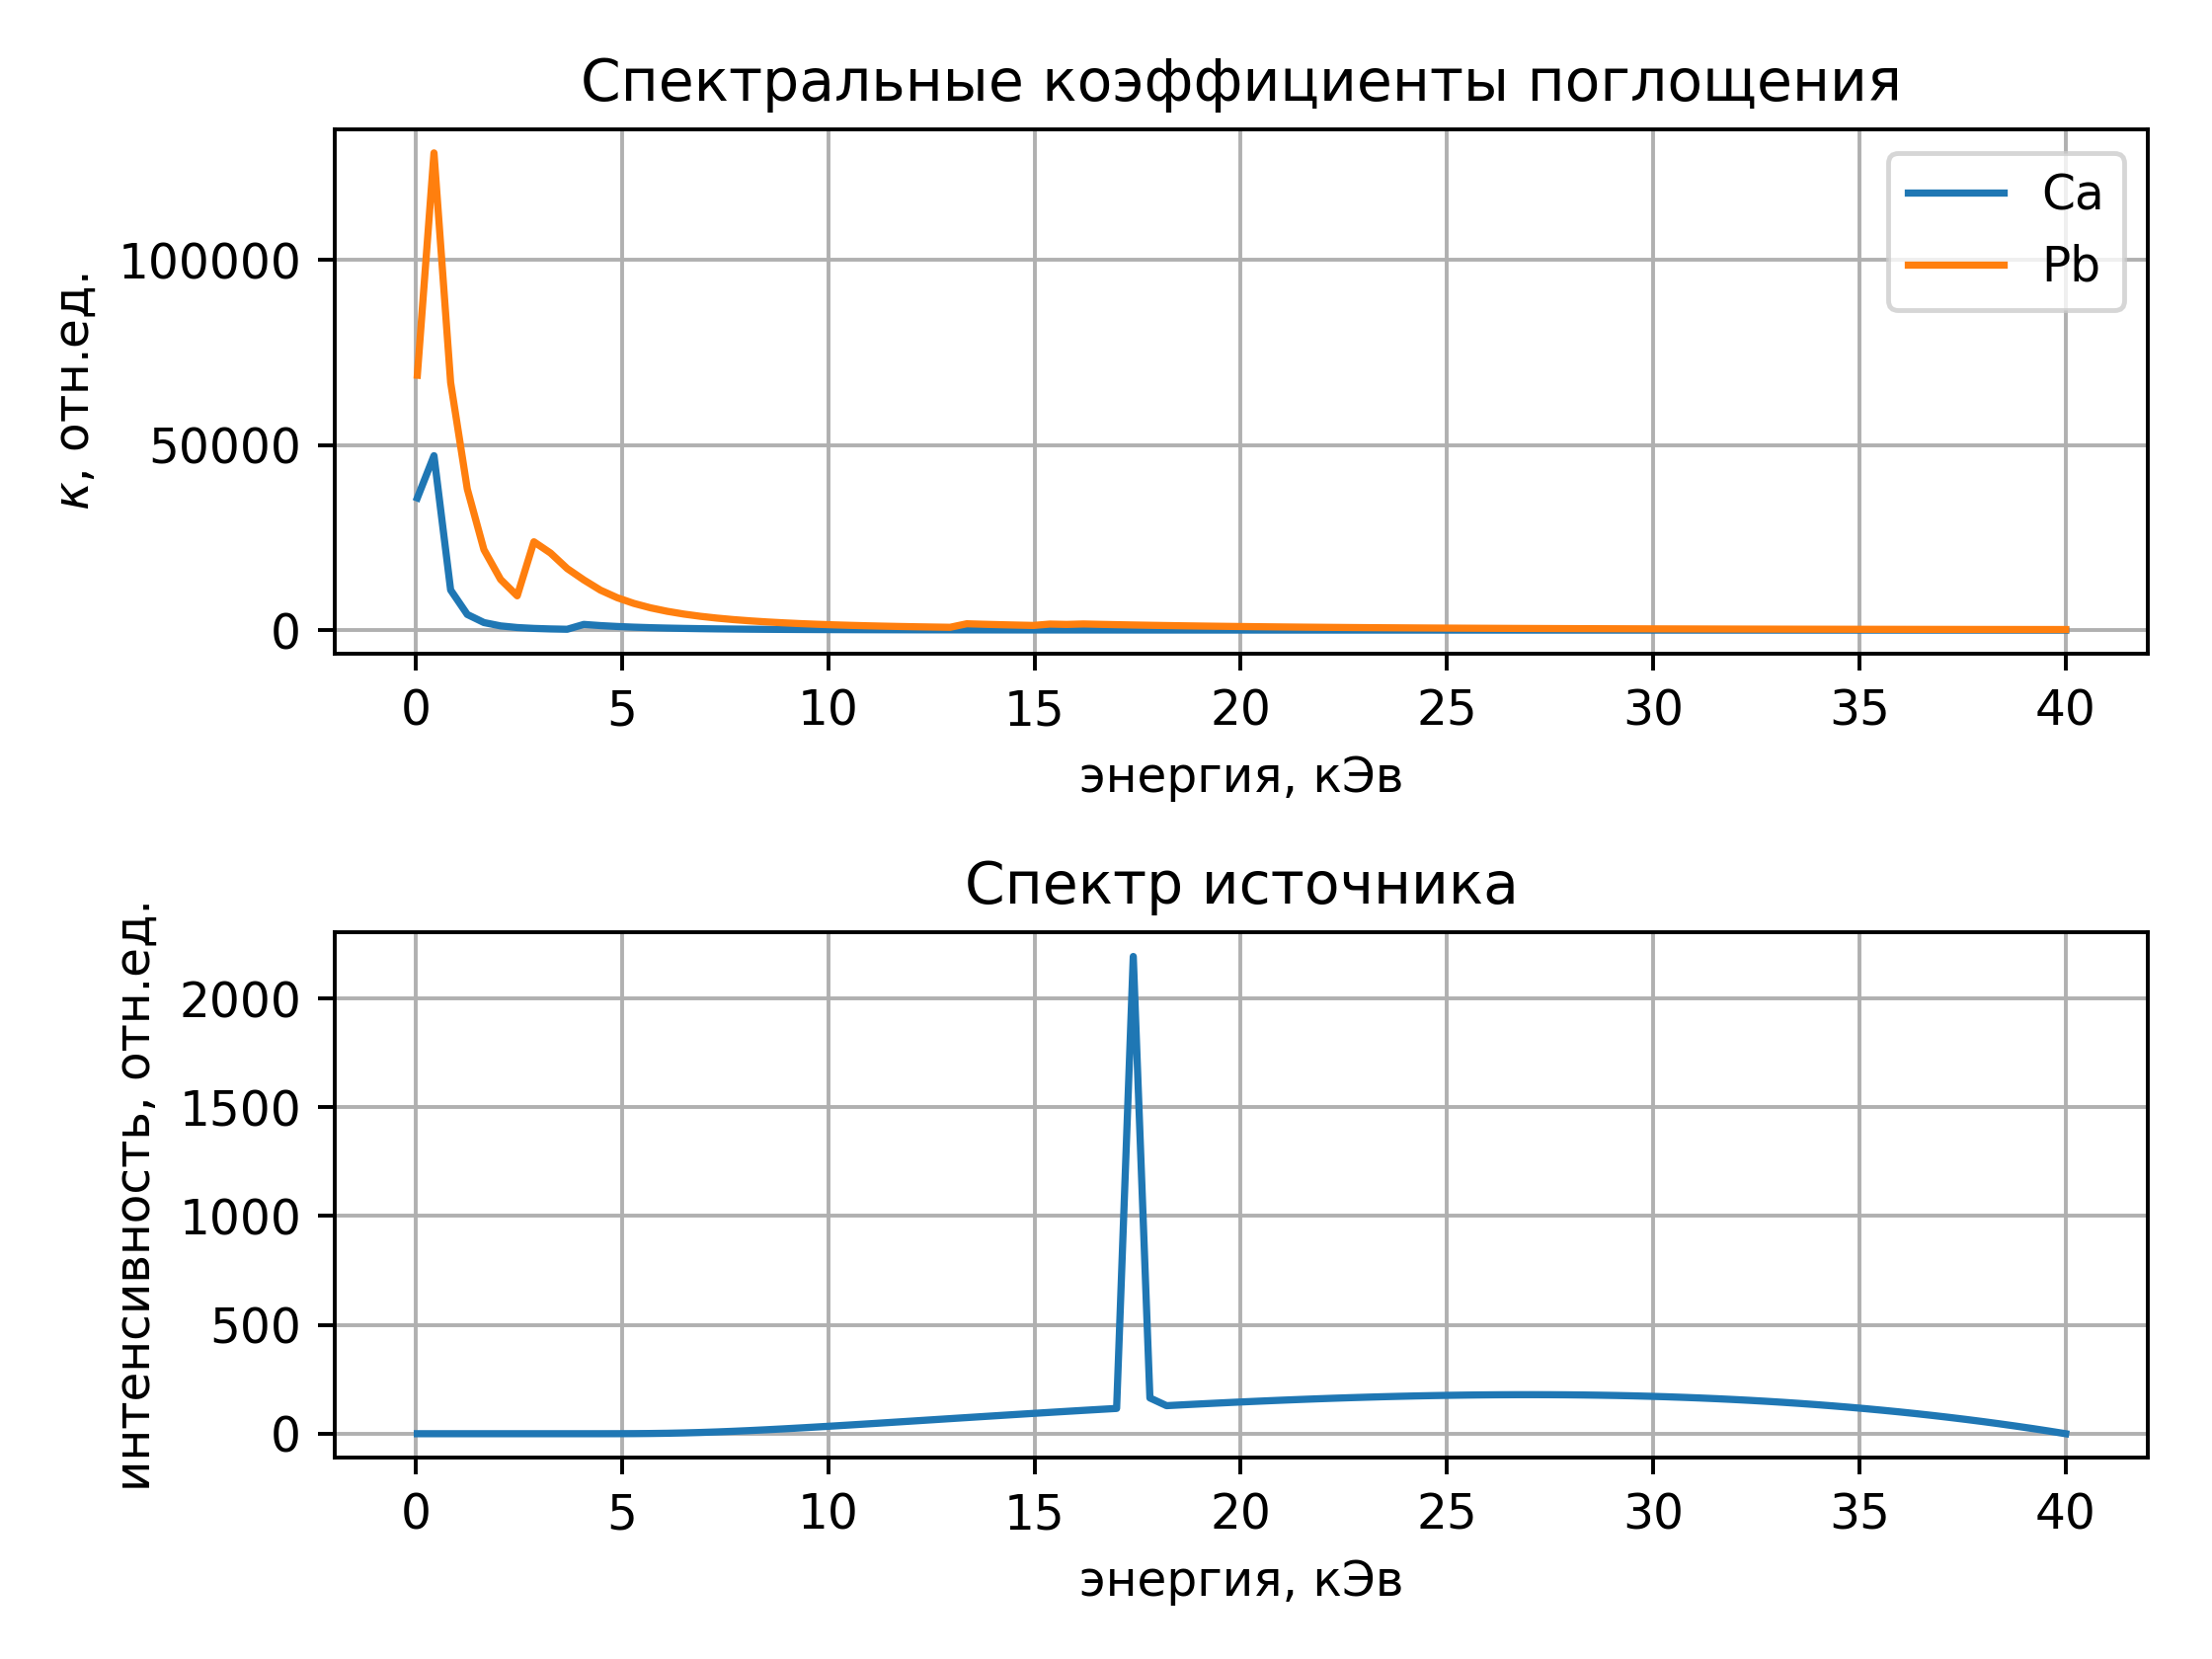
\includegraphics[width=\textwidth]{part2_img/zub_spectre} \\
    \caption{сверху: спектральные функции ослабления рентегновского излучения для кальция (Ca) и свинца (Pb) в относительных единицах. Снизу: спектр испускания молибденового анода}
    \label{fig:zub_spectre}
\end{figure}

Измерения проводились с помощью двумерного позиционно чувтсвительного рентгеновского детектора, разрешением $2000 \times 1250$ пикселей.
Измерялсось 400 проекционных углов от \ang{0} до \ang{199.5} с шагом в \ang{0.5}.
Данные измерены с избыточностью, угловой ``перехлест'' на \ang{30} обеспечивает возможность частичной корректировки ошибок, увеличивая количество уравнений в исходной задаче МНК для восстановления алгебраическими методами.
Перед восстановлением данные были подвергнуты предобработке.
Во-первых, был выделен регион интереса шириной в 1184 пикслея, содержащий исследуемый объект.
Эта операция лишь обрезает фон, то есть зоны нулевого поглощения на всех промеренных углах проекции, уменьшая размерность задачи и не теряя информации об объекте или разрешения.
Так же были проведены коррекции на сдвиг оси вращения и нормировка, интерполяция измерений в ``битых'' пикселях.

Исходные данные, полученные после измерений, составляют трехмерный тензор вещественных значений размера $400 \times 1184 \times 1049$.
В рамках данной работы рассматриваются восстановления измерений в плоском 2D сечении.
В данной главе будет рассмотрено сечение на высоте 820 пикс (отсчитывая сверху) от измеренного тензора.
На рис. \ref{fig:sino_zub}а представлено 2D измеренные показания детектора для одного угла проекции.
Линиями на рис. \ref{fig:sino_zub}а,в,г обозначена используемая линия уровня 820.
Полный вид синограммы вдоль одной линии, использованной для восстановлений, представлен на рис. \ref{fig:sino_zub}б.
Для проведения численных экспериментов по восстановлению, были использованы данные меньшего разрешения, полученные с использованием площадной интерполяции по смещению и интерполяции ``по ближайшему соседу'' по углу.
В частности рассматриваются восстановления измерений размерами $180 \times 128$ и $360 \times 256$ пикселей.

\begin{figure}
    \centering
    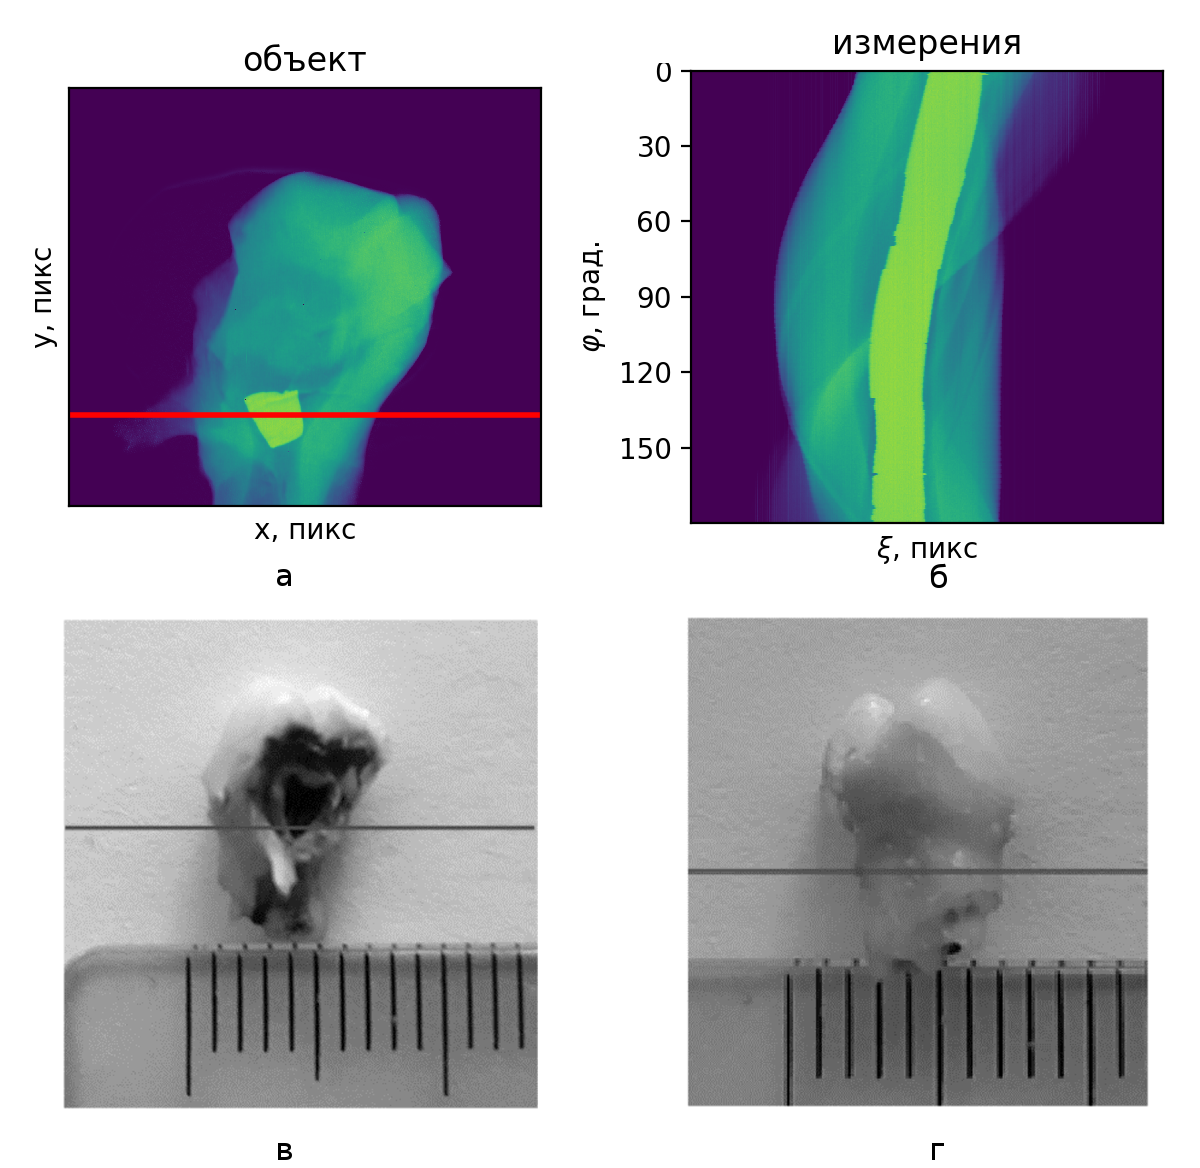
\includegraphics[width=0.9\textwidth]{part2_img/sino_zub} \\
    \caption{a) 2D-измерения для угла \ang{180}. б) полная синограмма для 1D-сечения. в), г) фотографии использованного образца рядом с 1-мм шкалой}
    \label{fig:sino_zub}
\end{figure}

Для использования методов на основе модели неравенств \ref{eq:quadprog_ineq}, рассматриваемых в этой главе, необходим выбор порогового значения $\delta$.
В предыдущих рассмотренных примерах использовалось модельное значение порога, примененное в симуляциях, на основе которых и были проведены восстановления.
При работе с реальными данными значение порога можно выбрать на основе анализа измерений.
В частности, была построена гистрограмма интенсивностей, и порог был выбирался так, чтобы отсечь первый максимум гистограммы.


\section{Результаты восстановления}
Метод мягких ограничений был применен для восстановления измеренных данных как уменьшенного размера, так и исходного.
Для восстановления на уменьшенных данных в качестве оптимизационной процедуры использовался метод градиентного спуска с малым значением релаксационного параметра, в то время как на исходном изображении применялся метод сопряженных градиентов. 
Выбор заведомо хуже сходящейся оптимизационной процедуры обусловлен возможностью тонкого контроля за ходом оптимизации.

\begin{figure}
    \centering
    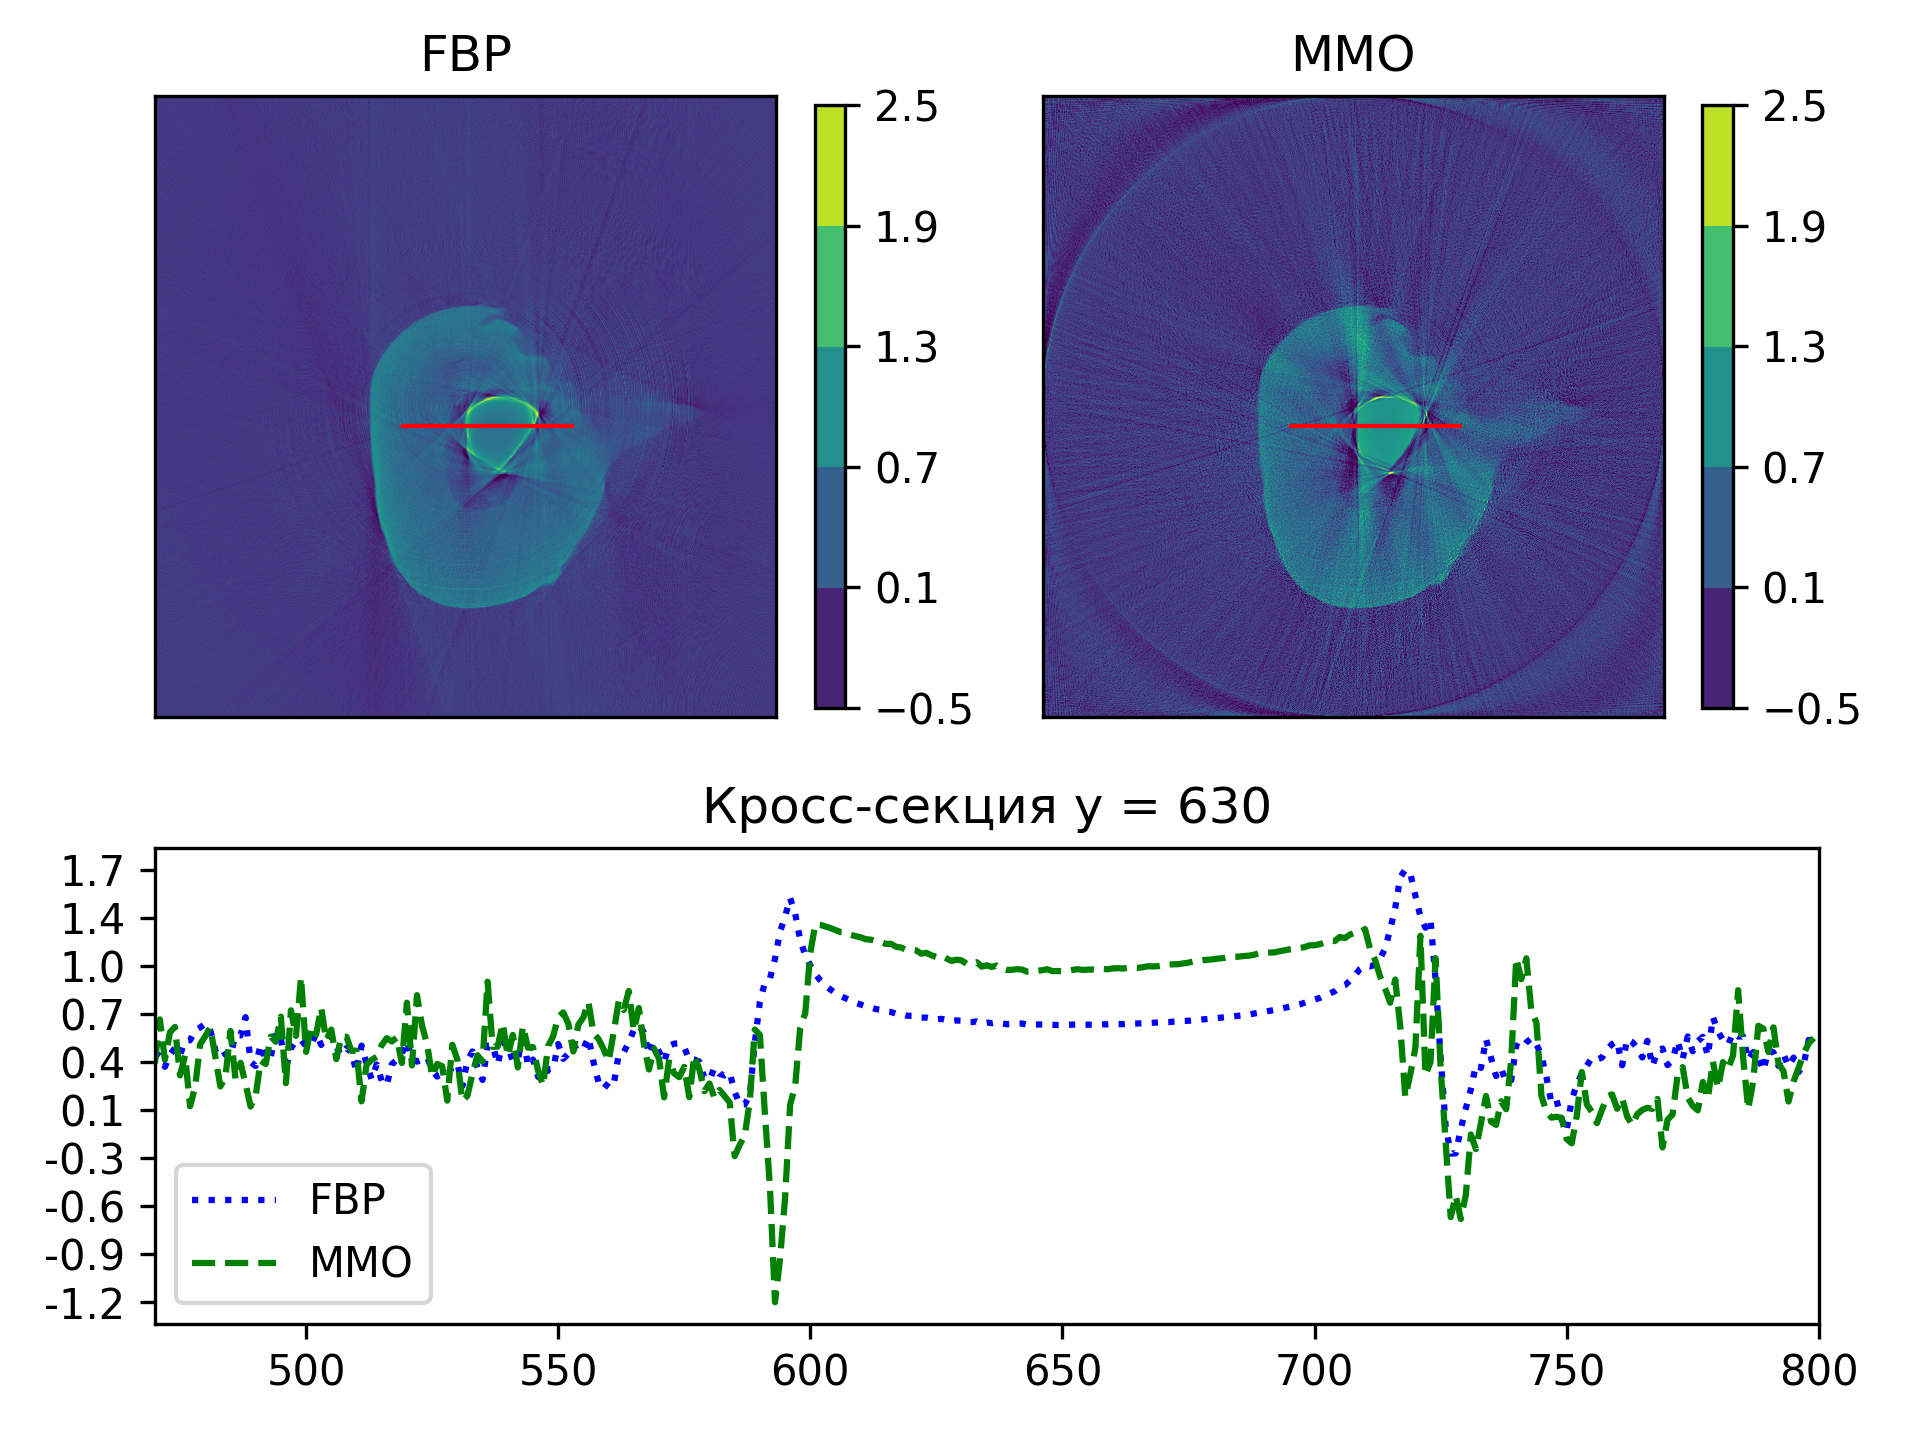
\includegraphics[width=1.0\textwidth]{part2_img/pb_big__fbp_vs_soft__cs__viridis} \\
    \caption{Результаты восстановления экспериментальных измерений методами свертки и обратной проекции (FBP) и мягких ограничений (ММО). Снизу представлены кросс-секции вдоль уровня y=630}
    \label{fig:fbp_vs_soft__zub}
\end{figure}

Результаты восстановления методами свертки и обратной проекции и мягких ограничений представлены на рисунке \ref{fig:fbp_vs_soft__zub}.
Восстановления обоими методами содержат шум и артефакты восстановления в виде полос ложной интенсивности.
При этом уровень включения (рис. \ref{fig:fbp_vs_soft__zub} снизу) восстановлен обоими методами по-разному.
Метод FBP не владеет информацией о сильном поглощении металлического включения, поэтому в районе включения возникает так называемый эффект чаши или cupping artifact (высокая интенсивность на границах включения с провалом к центру).
Метод мягких ограничений (ММО) же позволяет обеспечить ровную линию уровня вдоль включения, хотя восстановленная картина оказывается чуть более шумной.

Наличие линейных артефактов при восстановлении может быть вызвано неточностью в измерениях: на синограмме рис. \label{fig:sino_zub} б) виден ``скачок'' границы изображения включения.
На анимации 2D-измерений в этот момент четко видно, как металлическое включение сдвинулось относительно остального зуба.
То есть часть артефактов вызвана тем, что структура объекта поменялась в процессе измерений: часть измерений описывают состояние объекта до движения включения, а часть - после.

\section{Выводы}

